
\documentclass[11pt]{article}
\usepackage[margin=1in]{geometry}
\usepackage{amsmath}
\usepackage{booktabs}
\usepackage{graphicx}
\usepackage{float}
\usepackage{caption}
\usepackage[hidelinks]{hyperref}
\usepackage{tikz}
\usetikzlibrary{positioning,fit,arrows.meta,calc}

\newcommand{\invlogit}{\operatorname{logit}^{-1}}
\newcommand{\code}[1]{\texttt{#1}}

\graphicspath{{Plots_B/Convergence_Plots_B/}}

\title{Convergence Simulations Model B}
\author{Vera Schroeder}
\date{October 2026}

\begin{document}

\maketitle


\section{Model Structure}
\subsection{Data and indexing}
The data are $N$ binary trials. Trial $i$ has
\begin{itemize}
  \item a response $y_i \in \{0,1\}$, the monkey's categorization of the stimulus as ``low'' (0) or ``high'' (1);
  \item a standardized stimulus amplitude $x_i$. The raw amplitudes are centered and scaled by the mean and standard deviation of the distinct amplitude levels. The covariate row is
        $(1, x_i)$;
  \item a group $g[i] \in \{1,\dots,4\}$: the combination of
        hand and distractor condition,
        \[
          g \in \{\text{left\_uni},\ \text{left\_bi},\ \text{right\_uni},\ \text{right\_bi}\},
        \]
        where ``uni'' is unimanual (no distractor) and ``bi'' is bimanual
        (distractor present);
  \item a session $s[i] \in \{1,\dots,S\}$; the real data have
        $S = 42$.
\end{itemize}

\subsection{Likelihood}


Each response is Bernoulli,
\[
  y_i \sim \text{Bernoulli}(\psi_i), \qquad
  \psi_i = \psi\big(x_i;\ \theta_{g[i],s[i]}\big),
\]
with the psychometric function
\[
  \psi(x;\theta) = \gamma_h + (1 - \gamma_h - \gamma_l)\,\invlogit(\beta_0 + \beta_1 x),
  \qquad \theta = (\beta_0, \beta_1, \gamma_h, \gamma_l).
\]
Here $\beta_0$ and $\beta_1$ are parameters of the sigmoid, and $\gamma_h,\gamma_l$
set the asymptotes:
\[
  \lim_{x\to-\infty}\psi = \gamma_h, \qquad \lim_{x\to+\infty}\psi = 1-\gamma_l .
\]
So $\gamma_h$ is the probability of responding 1 (``high'') at very low amplitudes, and
$\gamma_l$ the probability of responding 0 (``low'') at very high amplitudes. In the code
$\psi_i$ is clipped to $[10^{-8},\,1-10^{-8}]$ before entering the Bernoulli
likelihood, for numerical stability.

\subsection{Session-level}

For each group $g$ and session $s$, the four parameters are drawn independently
from group-specific distributions:
\begin{align*}
  \beta_{0,gs} &\sim \mathcal{N}\big(\mu_{\beta_0,g},\ \sigma_{\beta_0,g}\big), \\
  \beta_{1,gs} &\sim \mathcal{N}\big(\mu_{\beta_1,g},\ \sigma_{\beta_1,g}\big), \\
  \gamma_{h,gs} &= 0.25\, w_{h,gs}, \qquad
      w_{h,gs} \sim \text{LogitNormal}\big(\mu_{\gamma_h,g},\ \sigma_{\gamma_h,g}\big), \\
  \gamma_{l,gs} &= 0.25\, w_{l,gs}, \qquad
      w_{l,gs} \sim \text{LogitNormal}\big(\mu_{\gamma_l,g},\ \sigma_{\gamma_l,g}\big).
\end{align*}
The LogitNormal keeps $w \in (0,1)$, so each lapse parameter $\gamma$ lies in
$(0, 0.25)$. That range keeps the curve increasing and makes the PSE and JND
below well defined.

Groups are independent of each other (no pooling across groups).

\subsection{Group-level Hyperpriors}

Each of the four groups has its own 8 hyperparameters, with the same priors in
every group:
\begin{align*}
  \mu_{\beta_0,g} &\sim \mathcal{N}(0,\ 2), &
  \sigma_{\beta_0,g} &\sim \text{HalfNormal}(2), \\
  \mu_{\beta_1,g} &\sim \text{LogNormal}(\log 4,\ 0.5), &
  \sigma_{\beta_1,g} &\sim \text{Exponential}(\lambda = 1) \quad (\text{mean } 1), \\
  \mu_{\gamma_h,g},\ \mu_{\gamma_l,g} &\sim \mathcal{N}(-3,\ 1.5), &
  \sigma_{\gamma_h,g},\ \sigma_{\gamma_l,g} &\sim \text{HalfNormal}(0.5).
\end{align*}
All hyperparameters are independent. The priors were chosen from the stimulus
design and general knowledge of the task, and checked by prior predictive
simulation (\code{Check\_Prior\_B.py}), not from fits to the real data:
\begin{itemize}
  \item $\mu_{\beta_0}$: the stimulus amplitudes (6 to 50) are symmetric around 28,
        the category boundary, which standardizes to $x = 0$. This prior puts a
        group's typical PSE between amplitudes 13 and 43 with 90\% probability,
        and outside the stimulus range only 3\% of the time.
  \item $\sigma_{\beta_0}$: weakly informative, bounded by the design. The implied
        day-to-day sd of the PSE has median about 5 amplitude units and is below
        about 20 with 95\% probability, small next to the stimulus range.
  \item $\mu_{\beta_1}$: positive with no upper bound; median 4, 95\% in
        $[1.5,\ 10.6]$.
  \item $\sigma_{\beta_1}$: mean 1, so that sessions vary around the group slope
        without the session slopes turning negative (2\% prior probability).
  \item $\mu_\gamma$ (logit scale): the typical lapse rate
        $0.25\,\invlogit(\mu_\gamma)$ has median 0.012 and 95\% range
        $[0.0007,\ 0.12]$; trained animals lapse on a few percent of trials and
        rarely more than about 10\%.
  \item $\sigma_\gamma$ (logit scale): median 0.34. For a group whose typical
        lapse rate is 0.05, this puts about 80\% of sessions between 0.03 and 0.07.
\end{itemize}

An earlier version of the model used
$\mu_{\beta_0} \sim \mathcal{U}[-12,\ 12]$,
$\sigma_{\beta_0} \sim \text{Exponential}(\text{mean } 12)$,
$\mu_{\beta_1} \sim \mathcal{U}[0,\ 8]$,
$\sigma_{\beta_1} \sim \text{Exponential}(\text{mean } 4)$,
$\mu_\gamma \sim \mathcal{N}(-2.5,\ 1)$ and
$\sigma_\gamma \sim \text{HalfNormal}(1.25)$.
Its convergence study motivated the changes (Section~\ref{sec:earlier}).

\subsection{Graphical Model}

\begin{center}
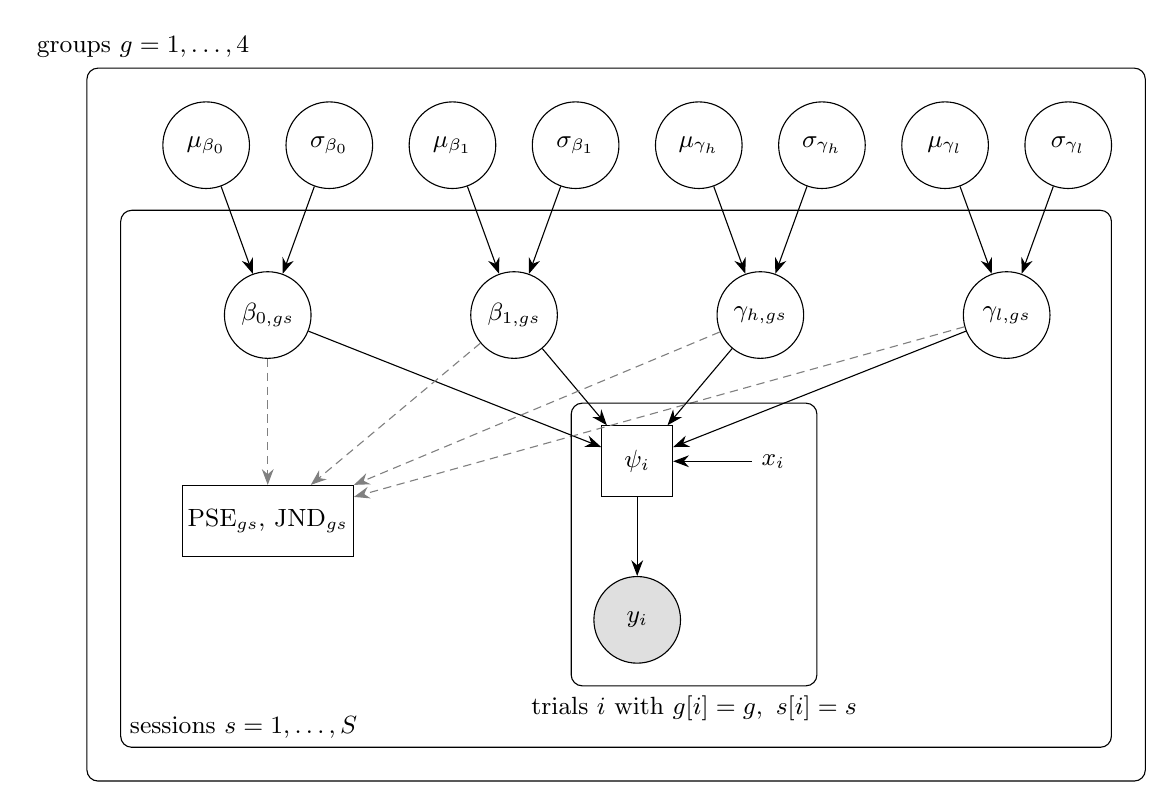
\begin{tikzpicture}[
    node distance=1.1cm and 0.45cm,
    latent/.style={circle, draw, minimum size=11mm, inner sep=0pt, font=\small},
    obs/.style={latent, fill=gray!25},
    det/.style={rectangle, draw, minimum size=9mm, inner sep=2pt, font=\small},
    const/.style={font=\small},
    arr/.style={-{Stealth[length=2mm]}},
    plate/.style={draw, rounded corners, inner sep=8pt}
  ]
  % hyperparameters
  \node[latent] (mub0) {$\mu_{\beta_0}$};
  \node[latent, right=of mub0] (sb0) {$\sigma_{\beta_0}$};
  \node[latent, right=of sb0] (mub1) {$\mu_{\beta_1}$};
  \node[latent, right=of mub1] (sb1) {$\sigma_{\beta_1}$};
  \node[latent, right=of sb1] (mugh) {$\mu_{\gamma_h}$};
  \node[latent, right=of mugh] (sgh) {$\sigma_{\gamma_h}$};
  \node[latent, right=of sgh] (mugl) {$\mu_{\gamma_l}$};
  \node[latent, right=of mugl] (sgl) {$\sigma_{\gamma_l}$};

  % session-level parameters
  \node[latent, below=1.6cm of $(mub0)!0.5!(sb0)$] (b0) {$\beta_{0,gs}$};
  \node[latent, below=1.6cm of $(mub1)!0.5!(sb1)$] (b1) {$\beta_{1,gs}$};
  \node[latent, below=1.6cm of $(mugh)!0.5!(sgh)$] (gh) {$\gamma_{h,gs}$};
  \node[latent, below=1.6cm of $(mugl)!0.5!(sgl)$] (gl) {$\gamma_{l,gs}$};

  % derived
  \node[det, below=1.6cm of b0] (pse) {PSE$_{gs}$, JND$_{gs}$};

  % trial level
  \node[det, below=1.4cm of $(b1)!0.5!(gh)$] (psi) {$\psi_i$};
  \node[obs, below=1.0cm of psi] (y) {$y_i$};
  \node[const, right=1.0cm of psi] (x) {$x_i$};

  \foreach \h/\p in {mub0/b0, sb0/b0, mub1/b1, sb1/b1, mugh/gh, sgh/gh, mugl/gl, sgl/gl}
    \draw[arr] (\h) -- (\p);
  \foreach \p in {b0, b1, gh, gl}
    \draw[arr] (\p) -- (psi);
  \foreach \p in {b0, b1, gh, gl}
    \draw[arr, densely dashed, gray] (\p) -- (pse);
  \draw[arr] (x) -- (psi);
  \draw[arr] (psi) -- (y);

  % plates
  \node[plate, fit=(x)(psi)(y), label={[font=\small]below:{trials $i$ with $g[i]=g,\ s[i]=s$}}] (ptrial) {};
  \node[plate, fit=(b0)(gl)(pse)(ptrial), inner sep=22pt,
        label={[font=\small, anchor=south west]south west:{sessions $s = 1,\dots,S$}}] (psess) {};
  \node[plate, fit=(mub0)(sgl)(psess), inner sep=12pt,
        label={[font=\small]above left:{groups $g = 1,\dots,4$}}] {};
\end{tikzpicture}
\end{center}

\noindent
Circles are random variables (shaded: observed), rectangles are deterministic
functions, and $x_i$ is a fixed covariate. Dashed arrows lead to derived
quantities that do not feed back into the likelihood.


\subsection{Derived Quantities: PSE and JND}

For each group and session the model records two summaries of the psychometric
curve.

\paragraph{Point of subjective equality (PSE):} the stimulus at which a response of ``high'' and ``low'' are equally likely ($\psi = 1/2$). Solving
$\psi(x;\theta) = \tfrac12$ for x gives
\[
  \text{PSE} = \frac{1}{\beta_1}\left[-\beta_0 + \log\frac{1-2\gamma_h}{1-2\gamma_l}\right].
\]

\paragraph{Just noticeable difference (JND):} the amount the stimulus must be changed for the
difference to be noticeable half of the time, a measure of sensitivity. This is computed as half the stimulus distance between the points where $\psi = 0.25$ and $\psi = 0.75$,
\[
  \text{JND} = \frac{x_{.75} - x_{.25}}{2}
  = \frac{1}{2\beta_1}\,\log\frac{(3-4\gamma_h)(3-4\gamma_l)}{(1-4\gamma_h)(1-4\gamma_l)} .
\]
Both are in units of the standardized stimulus. When
$\gamma_h=\gamma_l=0$, they reduce to $\text{PSE} = - \frac{\beta_0}{\beta_1} $ and $\text{JND} =  \frac{\log 3}{\beta_1}$.

\subsection{Implementation}

To aid fit, as in the convention of typical logistic regression, the raw amplitudes $x_i$ are centered and scaled by the mean and standard deviation of the distinct amplitude levels. To aid convergence of HMC NUTS, all distributions are written as deterministic transforms of a standard normal or uniform random variable. These non-centered parameterizations mean the sampler only works with uniform or standard normal variables.

\section{Synthetic Data Generation}

The true hyperparameters are the posterior means of Model B's fit to the real data
(\code{Results\_B.pkl}, from \code{Main\_Analysis\_B.py}; see the report ``Model B Fit
to the Real Data''), so the synthetic data resemble the real data
(Table~\ref{tab:true}). They only generate data; the priors do not use them. Each
replicate draws new session-level parameters from them.

\begin{table}[H]
\centering
\caption{True hyperparameters: posterior means of the real-data fit. The lapse-rate
ones are on the logit scale; the typical lapse rate is $0.25\,\invlogit(\mu_\gamma)$.}
\label{tab:true}
\begin{tabular}{lcccc}
\toprule
 & left\_uni & left\_bi & right\_uni & right\_bi \\
\midrule
$\mu_{\beta_0}$     & $-1.487$ & $-0.099$ & $-1.056$ & 0.686 \\
$\mu_{\beta_1}$     & 4.968 & 4.321 & 4.580 & 4.340 \\
$\mu_{\gamma_h}$    & $-5.203$ & $-2.350$ & $-4.729$ & $-1.816$ \\
$\mu_{\gamma_l}$    & $-3.445$ & $-3.442$ & $-3.717$ & $-3.228$ \\
$\sigma_{\beta_0}$  & 0.763 & 0.772 & 1.011 & 0.759 \\
$\sigma_{\beta_1}$  & 0.285 & 1.266 & 0.173 & 0.615 \\
$\sigma_{\gamma_h}$ & 0.359 & 0.591 & 0.371 & 0.362 \\
$\sigma_{\gamma_l}$ & 0.373 & 0.393 & 0.381 & 0.431 \\
\bottomrule
\end{tabular}
\end{table}

Compared with the earlier, hand-picked values (Section~\ref{sec:earlier}), these
have group slopes of 4.3--5.0 rather than 3 and 6, between-session sds of the slope
that are far from 0 (up to 1.27 for left\_bi), and unimanual $\gamma_h$ close to 0
(typical values 0.001--0.002).

The model was fit to 10 dataset conditions in two sweeps, each run twice with new data:
\begin{itemize}
  \item the sessions sweep varies the number of sessions (5, 10, 20, 40 and 80, each
        with 308 trials), mainly testing the hyperparameters;
  \item the trials sweep varies the trials per session (20, 40, 80, 160 and 320, with
        42 sessions), mainly testing the session-level parameters.
\end{itemize}
Within a replicate the datasets of a sweep are nested (the first $n$ sessions, or the
first $t$ trials of every session). The real data have 42 sessions with about 308
trials each, so the 40-session and 320-trial fits are the most representative.

\section{Model Fit Results}

Every figure and number in this report is produced by \code{Convergence\_B.py};
the cell ``Numbers for Convergence\_B\_Report.tex'' prints the numbers that the
earlier cells do not, and also runs on the saved results without refitting. The
statements about what the priors imply come from \code{Check\_Prior\_B.py}.
Hyperparameter entries are averaged over the two replicates; session-level RMSEs and
coverages are pooled over them (84 sessions per group in the trials sweep). The fits
sample the 4 chains in parallel; the whole study takes 0.7 hours.

\subsection{Sampling Diagnostics}
All 20 fits sampled without divergences, with $\hat{R} \le 1.011$ and a bulk ESS of at
least 670 for every hyperparameter, and $\hat{R} \le 1.007$ for every session-level
parameter.

\begin{table}[H]
\centering
\caption{Sampler diagnostics over both replicates. $\hat{R}$ and bulk ESS are
taken over the hyperparameters.}
\begin{tabular}{llccc}
\toprule
Sweep & Size & max $\hat{R}$ & min ESS & divergences \\
\midrule
sessions & 5   & 1.003 & 1503 & 0 \\
sessions & 10  & 1.005 & 1297 & 0 \\
sessions & 20  & 1.006 & 909  & 0 \\
sessions & 40  & 1.007 & 758  & 0 \\
sessions & 80  & 1.011 & 801  & 0 \\
\midrule
trials & 20  & 1.004 & 961  & 0 \\
trials & 40  & 1.005 & 1074 & 0 \\
trials & 80  & 1.006 & 822  & 0 \\
trials & 160 & 1.007 & 1000 & 0 \\
trials & 320 & 1.004 & 670  & 0 \\
\bottomrule
\end{tabular}
\end{table}

\subsection{Hyperparameter means}

\begin{figure}[H]
\centering
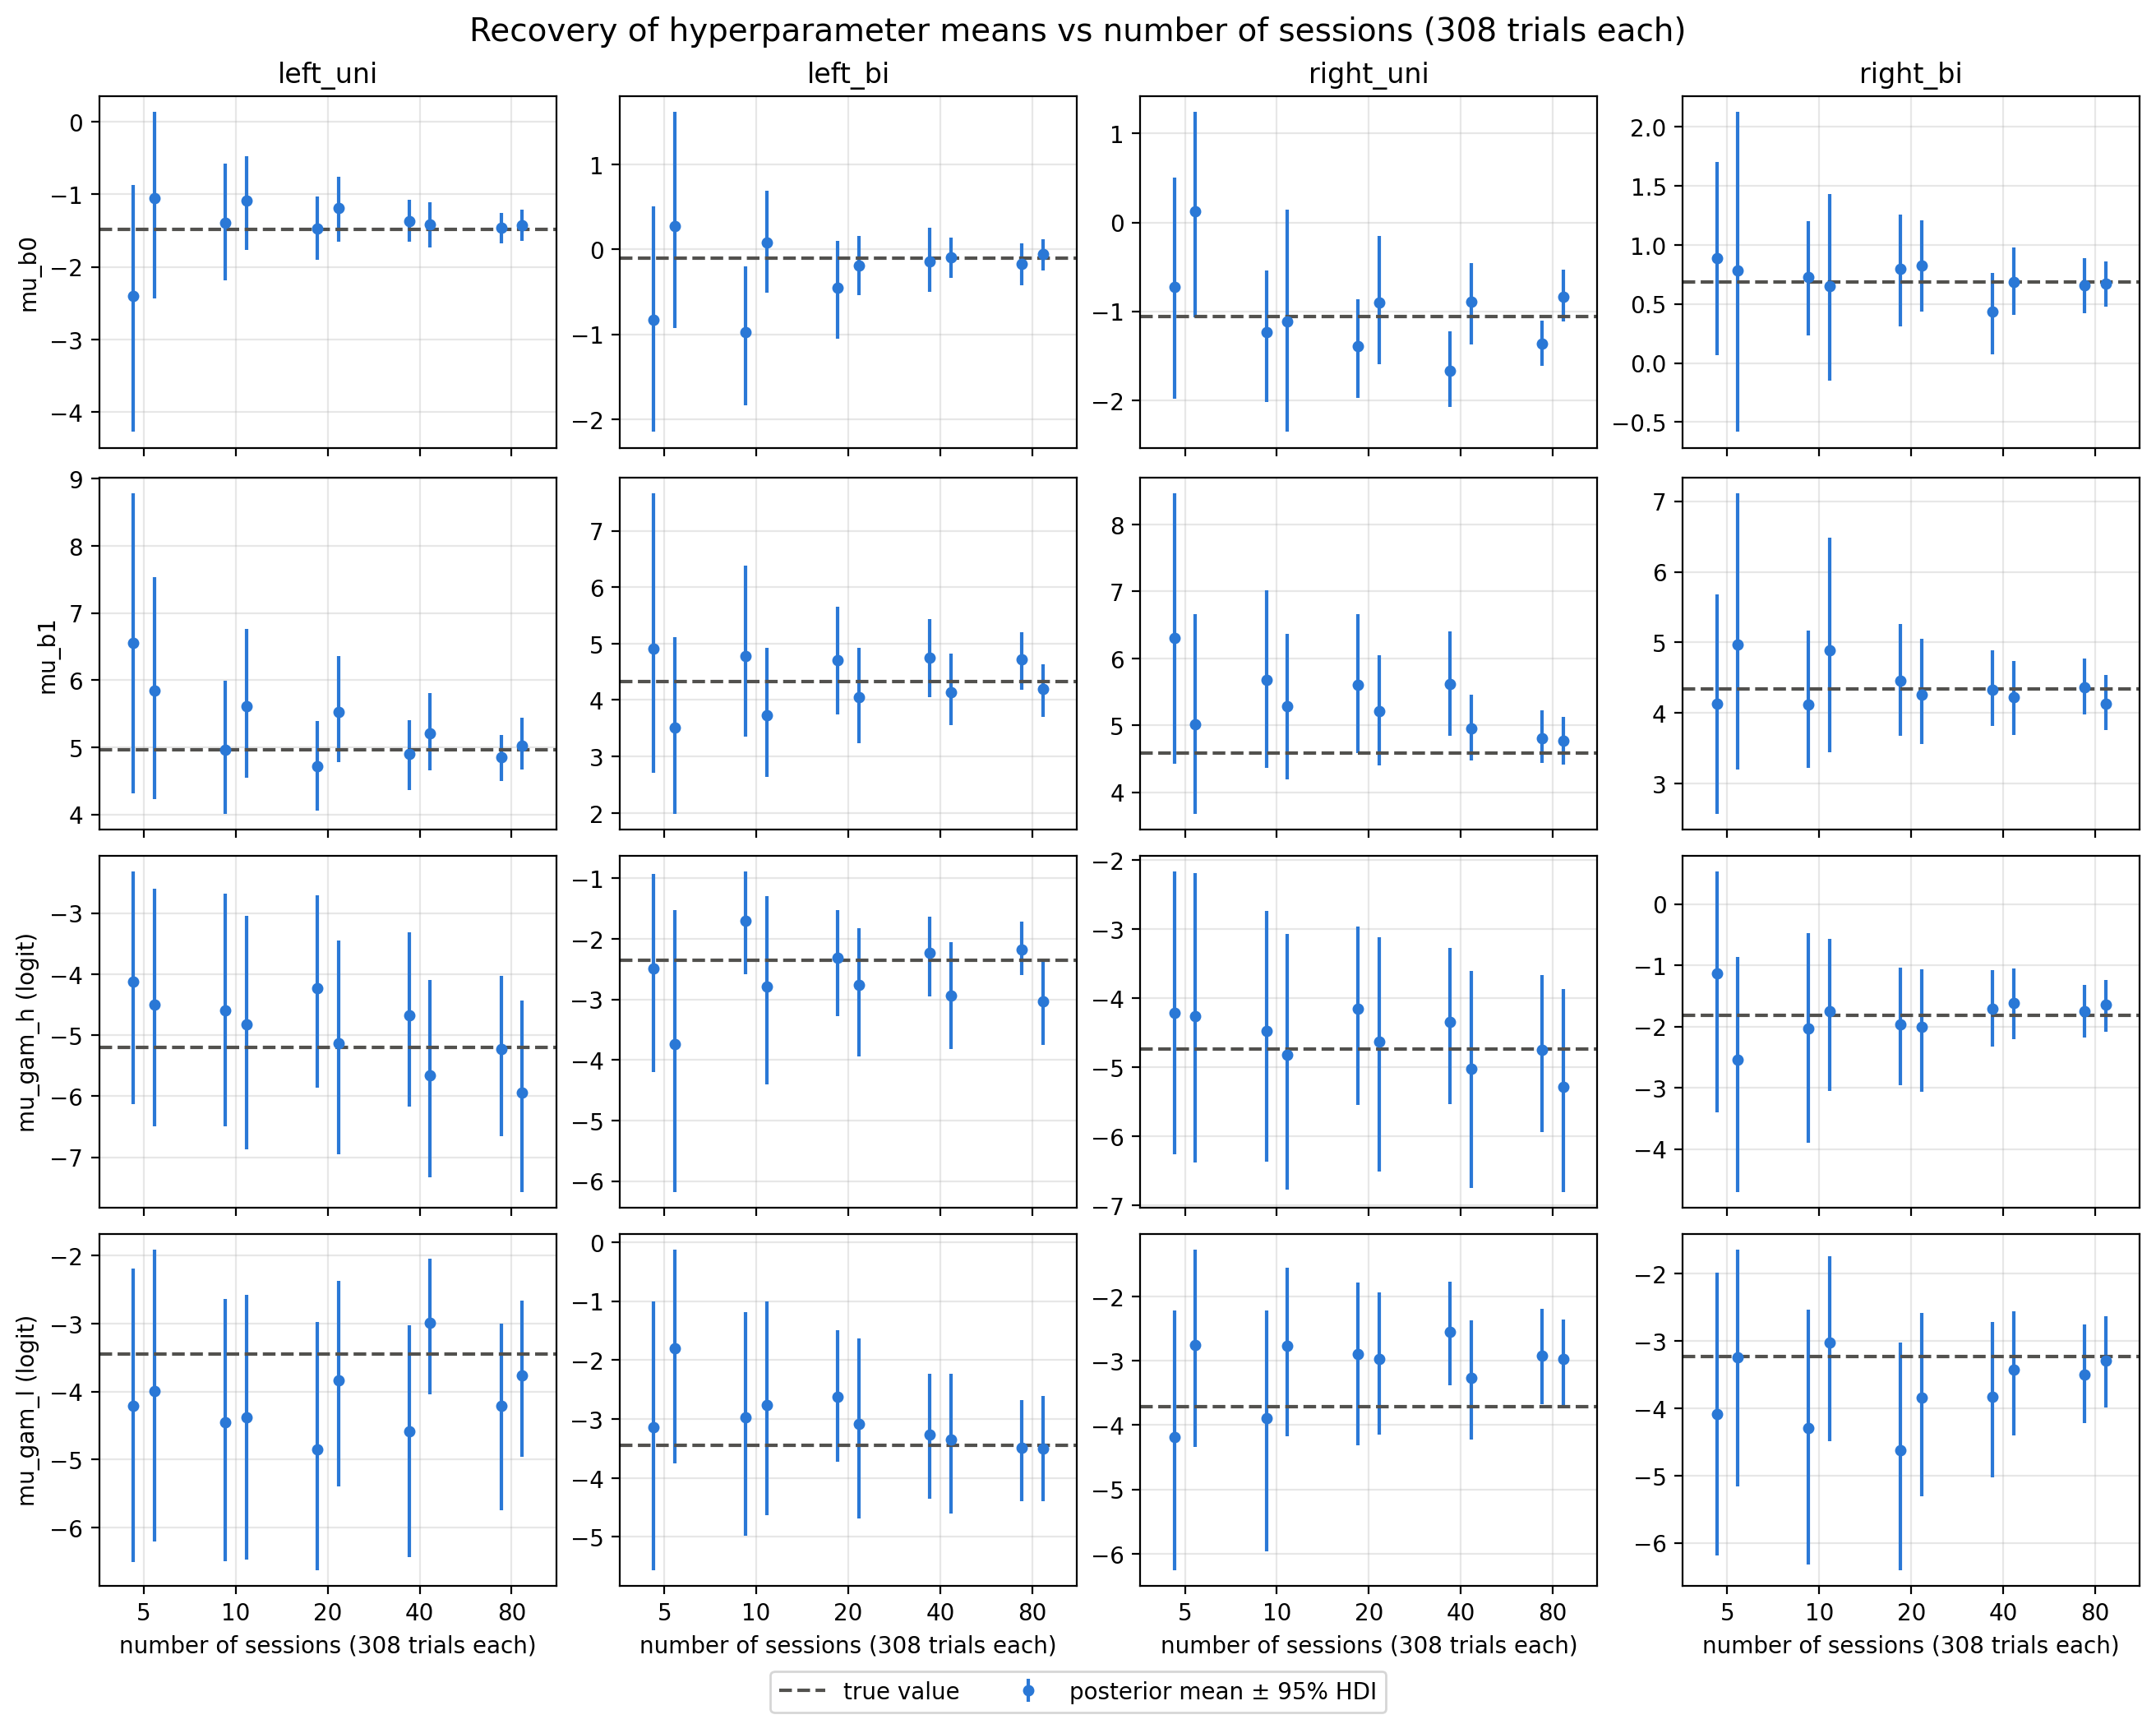
\includegraphics[width=\textwidth]{hyper_means_recovery_vs_sessions.png}
\caption{Posterior mean and 95\% HDI of the group means against the number of
sessions (308 trials each). The two replicates are drawn side by side; the
dashed line is the true value.}
\label{fig:means_sessions}
\end{figure}

\begin{figure}[H]
\centering
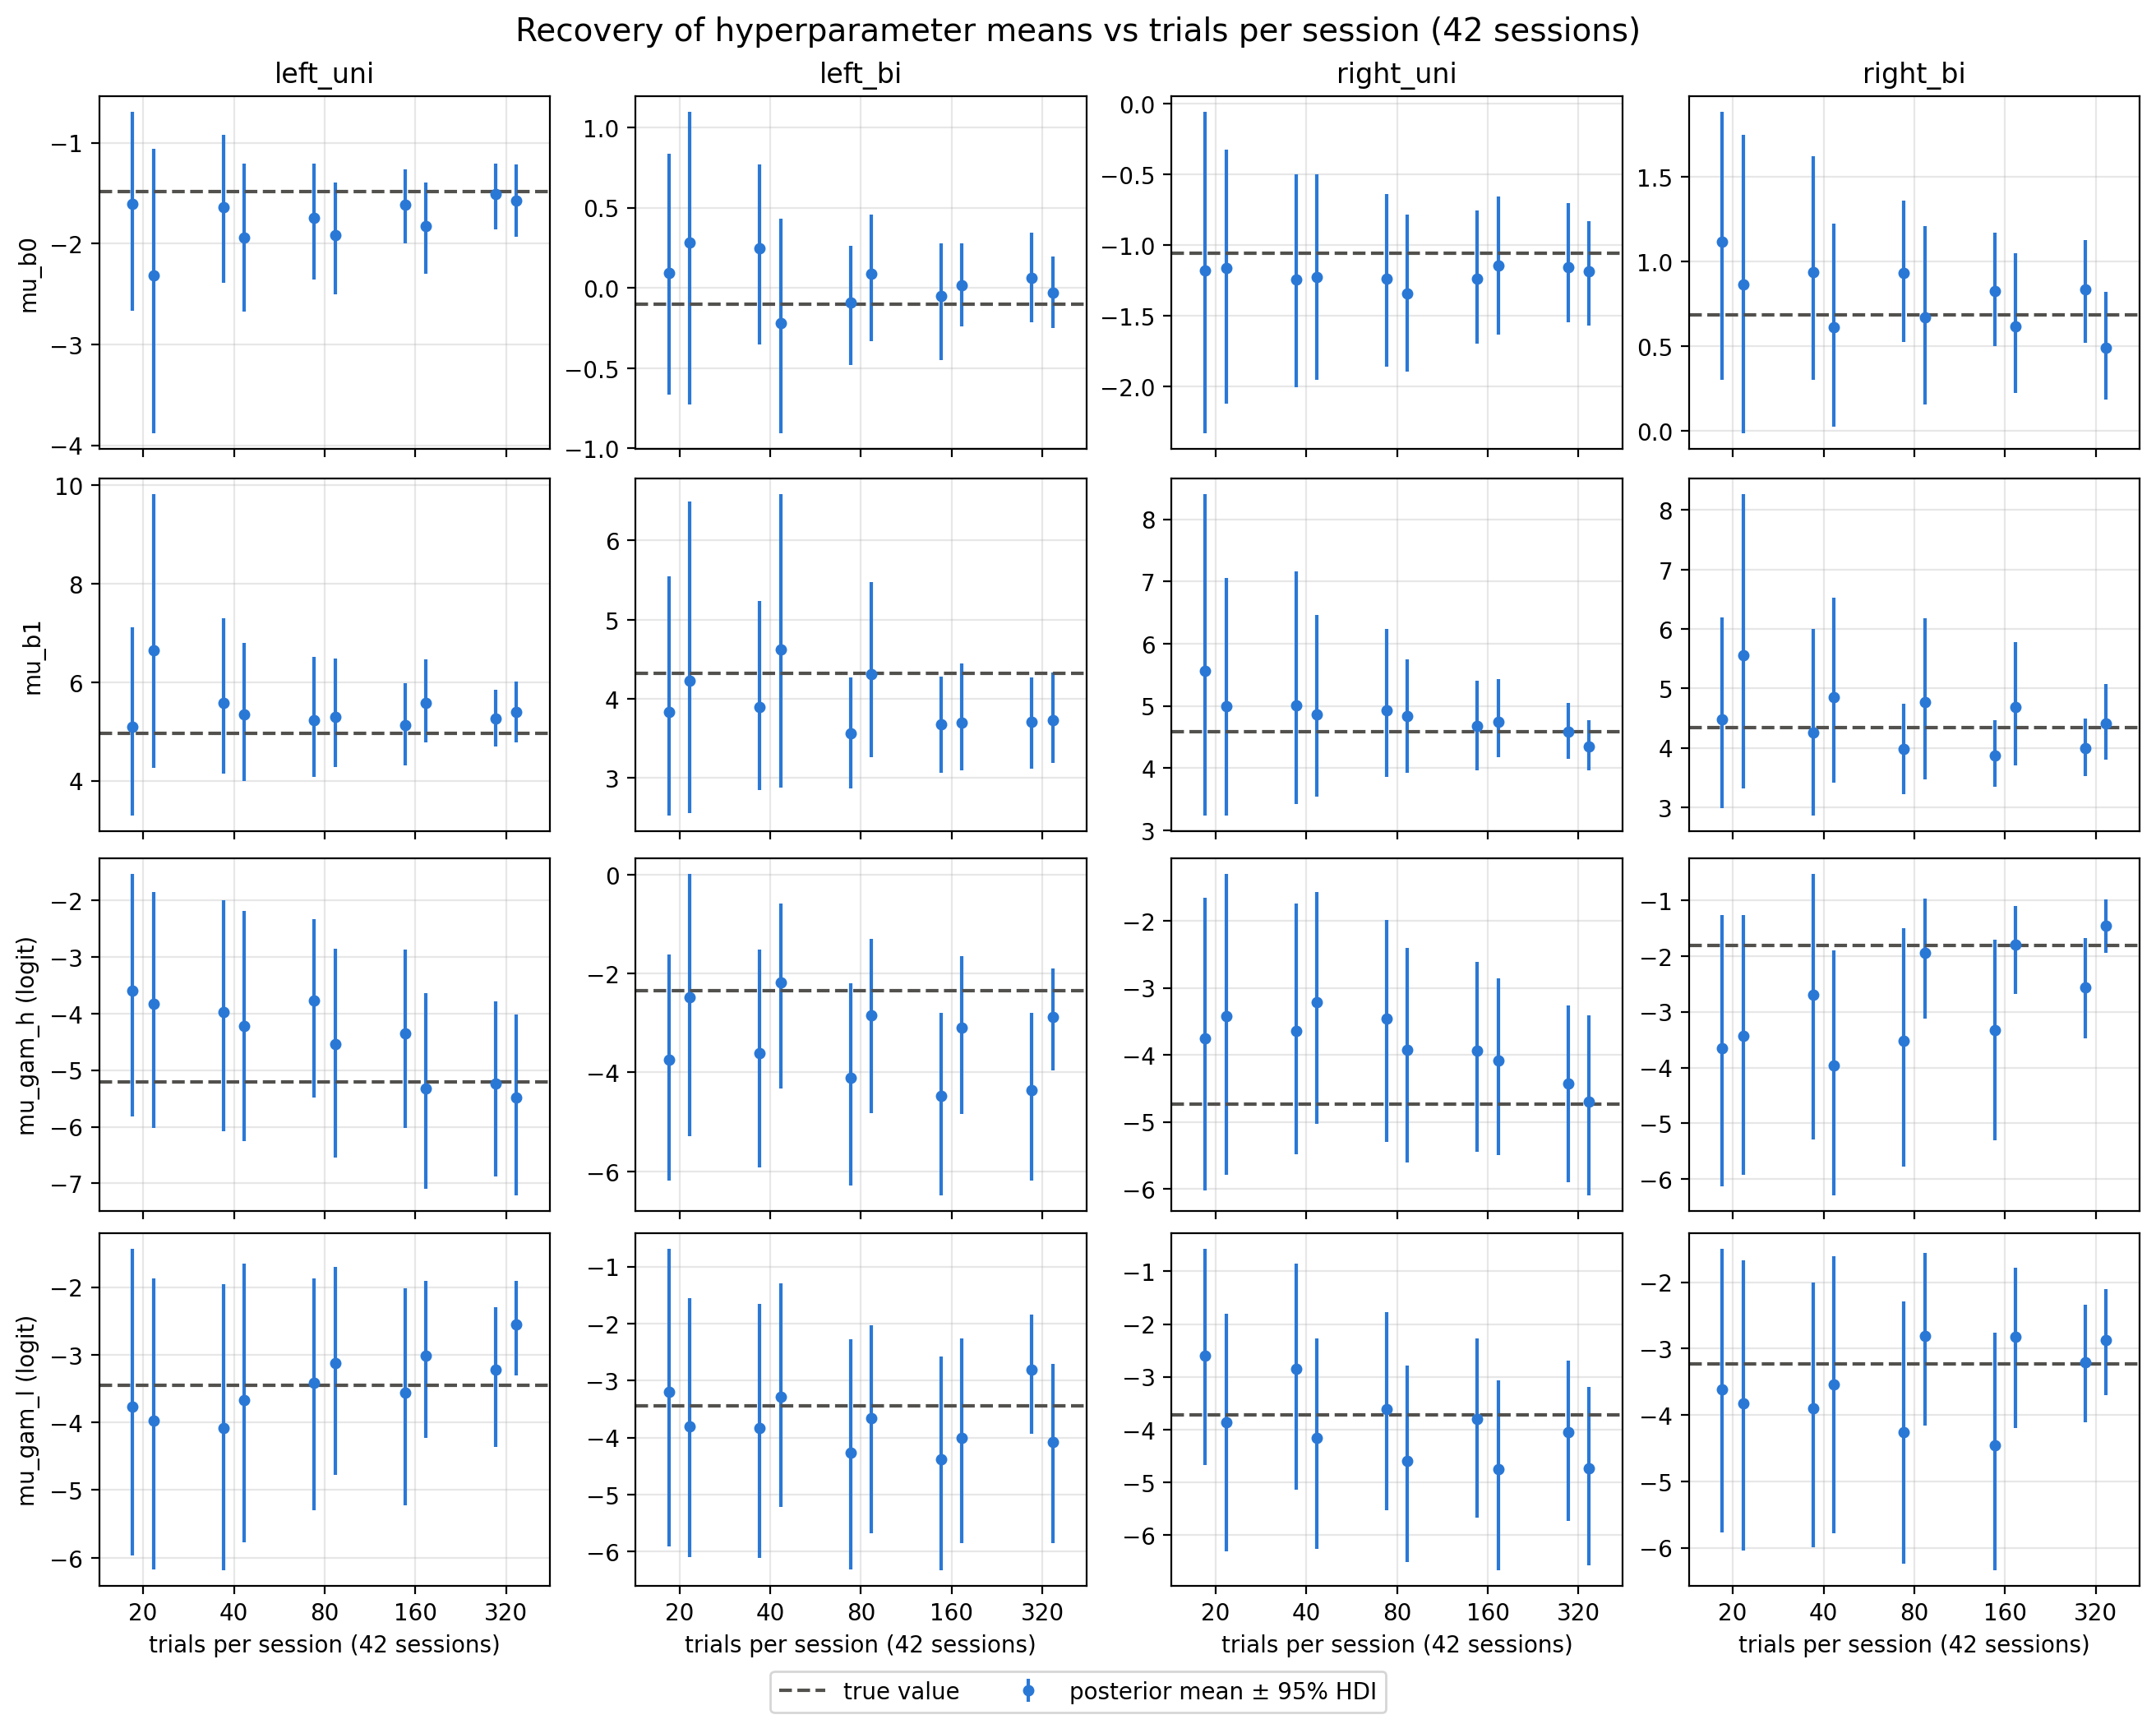
\includegraphics[width=\textwidth]{hyper_means_recovery_vs_trials.png}
\caption{As Figure~\ref{fig:means_sessions}, against trials per session (42
sessions).}
\label{fig:means_trials}
\end{figure}

\begin{table}[H]
\centering
\caption{Group means at 40 and 80 sessions (sessions sweep): true value and posterior
mean [95\% HDI], averaged over replicates. Lapse-rate means are on the logit scale.}
\label{tab:means}
\resizebox{\textwidth}{!}{%
\begin{tabular}{llcccc}
\toprule
 & & left\_uni & left\_bi & right\_uni & right\_bi \\
\midrule
$\mu_{\beta_0}$ & true & $-1.49$ & $-0.10$ & $-1.06$ & 0.69 \\
 & 40 & $-1.40$ [$-1.70$, $-1.09$] & $-0.12$ [$-0.42$, 0.20] & $-1.28$ [$-1.72$, $-0.84$] & 0.56 [0.24, 0.87] \\
 & 80 & $-1.44$ [$-1.66$, $-1.23$] & $-0.11$ [$-0.34$, 0.10] & $-1.10$ [$-1.36$, $-0.82$] & 0.66 [0.45, 0.87] \\
\midrule
$\mu_{\beta_1}$ & true & 4.97 & 4.32 & 4.58 & 4.34 \\
 & 40 & 5.06 [4.51, 5.61] & 4.44 [3.81, 5.13] & 5.29 [4.66, 5.93] & 4.27 [3.76, 4.82] \\
 & 80 & 4.94 [4.58, 5.31] & 4.46 [3.95, 4.92] & 4.79 [4.42, 5.18] & 4.25 [3.87, 4.65] \\
\midrule
$\mu_{\gamma_h}$ & true & $-5.20$ & $-2.35$ & $-4.73$ & $-1.82$ \\
 & 40 & $-5.17$ [$-6.75$, $-3.70$] & $-2.58$ [$-3.38$, $-1.84$] & $-4.68$ [$-6.13$, $-3.43$] & $-1.66$ [$-2.26$, $-1.07$] \\
 & 80 & $-5.58$ [$-7.11$, $-4.23$] & $-2.60$ [$-3.18$, $-2.02$] & $-5.01$ [$-6.37$, $-3.76$] & $-1.70$ [$-2.13$, $-1.28$] \\
\midrule
$\mu_{\gamma_l}$ & true & $-3.44$ & $-3.44$ & $-3.72$ & $-3.23$ \\
 & 40 & $-3.79$ [$-5.24$, $-2.54$] & $-3.31$ [$-4.48$, $-2.24$] & $-2.91$ [$-3.80$, $-2.08$] & $-3.63$ [$-4.71$, $-2.64$] \\
 & 80 & $-3.99$ [$-5.35$, $-2.83$] & $-3.49$ [$-4.40$, $-2.64$] & $-2.95$ [$-3.68$, $-2.28$] & $-3.40$ [$-4.11$, $-2.70$] \\
\bottomrule
\end{tabular}}
\end{table}

Over all 20 fits, the HDIs of the group means contain the true value in 94--96\% of
cases (Table~\ref{tab:means}).

\paragraph{Bias $\mu_{\beta_0}$:} Recovered in all groups. At 40 sessions the posterior
means are within 0.22 of the truth, with HDI widths of 0.61--0.88. For right\_uni one
of the two replicates misses the truth at 40 and at 80 sessions.

\paragraph{Slope $\mu_{\beta_1}$:} Recovered in all groups. At 80 sessions the posterior
means are within 0.21 of the truth and every HDI contains it. At 40 sessions the HDIs
are 1.06--1.32 wide, and right\_uni lies above the truth (5.29 against 4.58, one
replicate missing it). Unlike the earlier study, where a true slope of 6 was poorly
identified, the real slopes of 4.3--5.0 make the rise from $\psi = 0.25$ to 0.75 span
more than one stimulus spacing.

\paragraph{Lapse-rate means $\mu_{\gamma_h}$ and $\mu_{\gamma_l}$:} The least precise
means, because lapses are rare and show only where the sigmoid has reached its floor
or ceiling (about 3 expected $\gamma_l$ lapses per stimulus level for the left-hand
groups at the real data size). Their HDIs contain the truth in nearly every fit, but
three points stand out:
\begin{itemize}
  \item $\mu_{\gamma_h}$ of the unimanual groups, whose true typical $\gamma_h$ is
        0.001--0.002, has wide HDIs (2.7--3.1 at 40 sessions): with almost no lapses the data
        only say that $\gamma_h$ is small.
  \item $\mu_{\gamma_h}$ of left\_bi is too low in the trials sweep: $-3.62$
        [$-5.07$, $-2.35$] at 320 trials against a true $-2.35$. Its curve never
        reaches its floor within the stimulus range.
  \item $\mu_{\gamma_l}$ of right\_uni is too high: at 80 sessions $-2.95$
        [$-3.68$, $-2.28$] against a true $-3.72$, and both replicates' HDIs miss the
        truth. The earlier study found the same overestimate for this group, under
        both sets of priors and at different true values; its cause has not been
        identified.
\end{itemize}
$\mu_{\gamma_l}$ of left\_uni is also too high in the trials sweep ($-2.88$ against
$-3.44$ at 320 trials), though its HDI contains the truth.

\subsection{Hyperparameter standard deviations}

\begin{figure}[H]
\centering
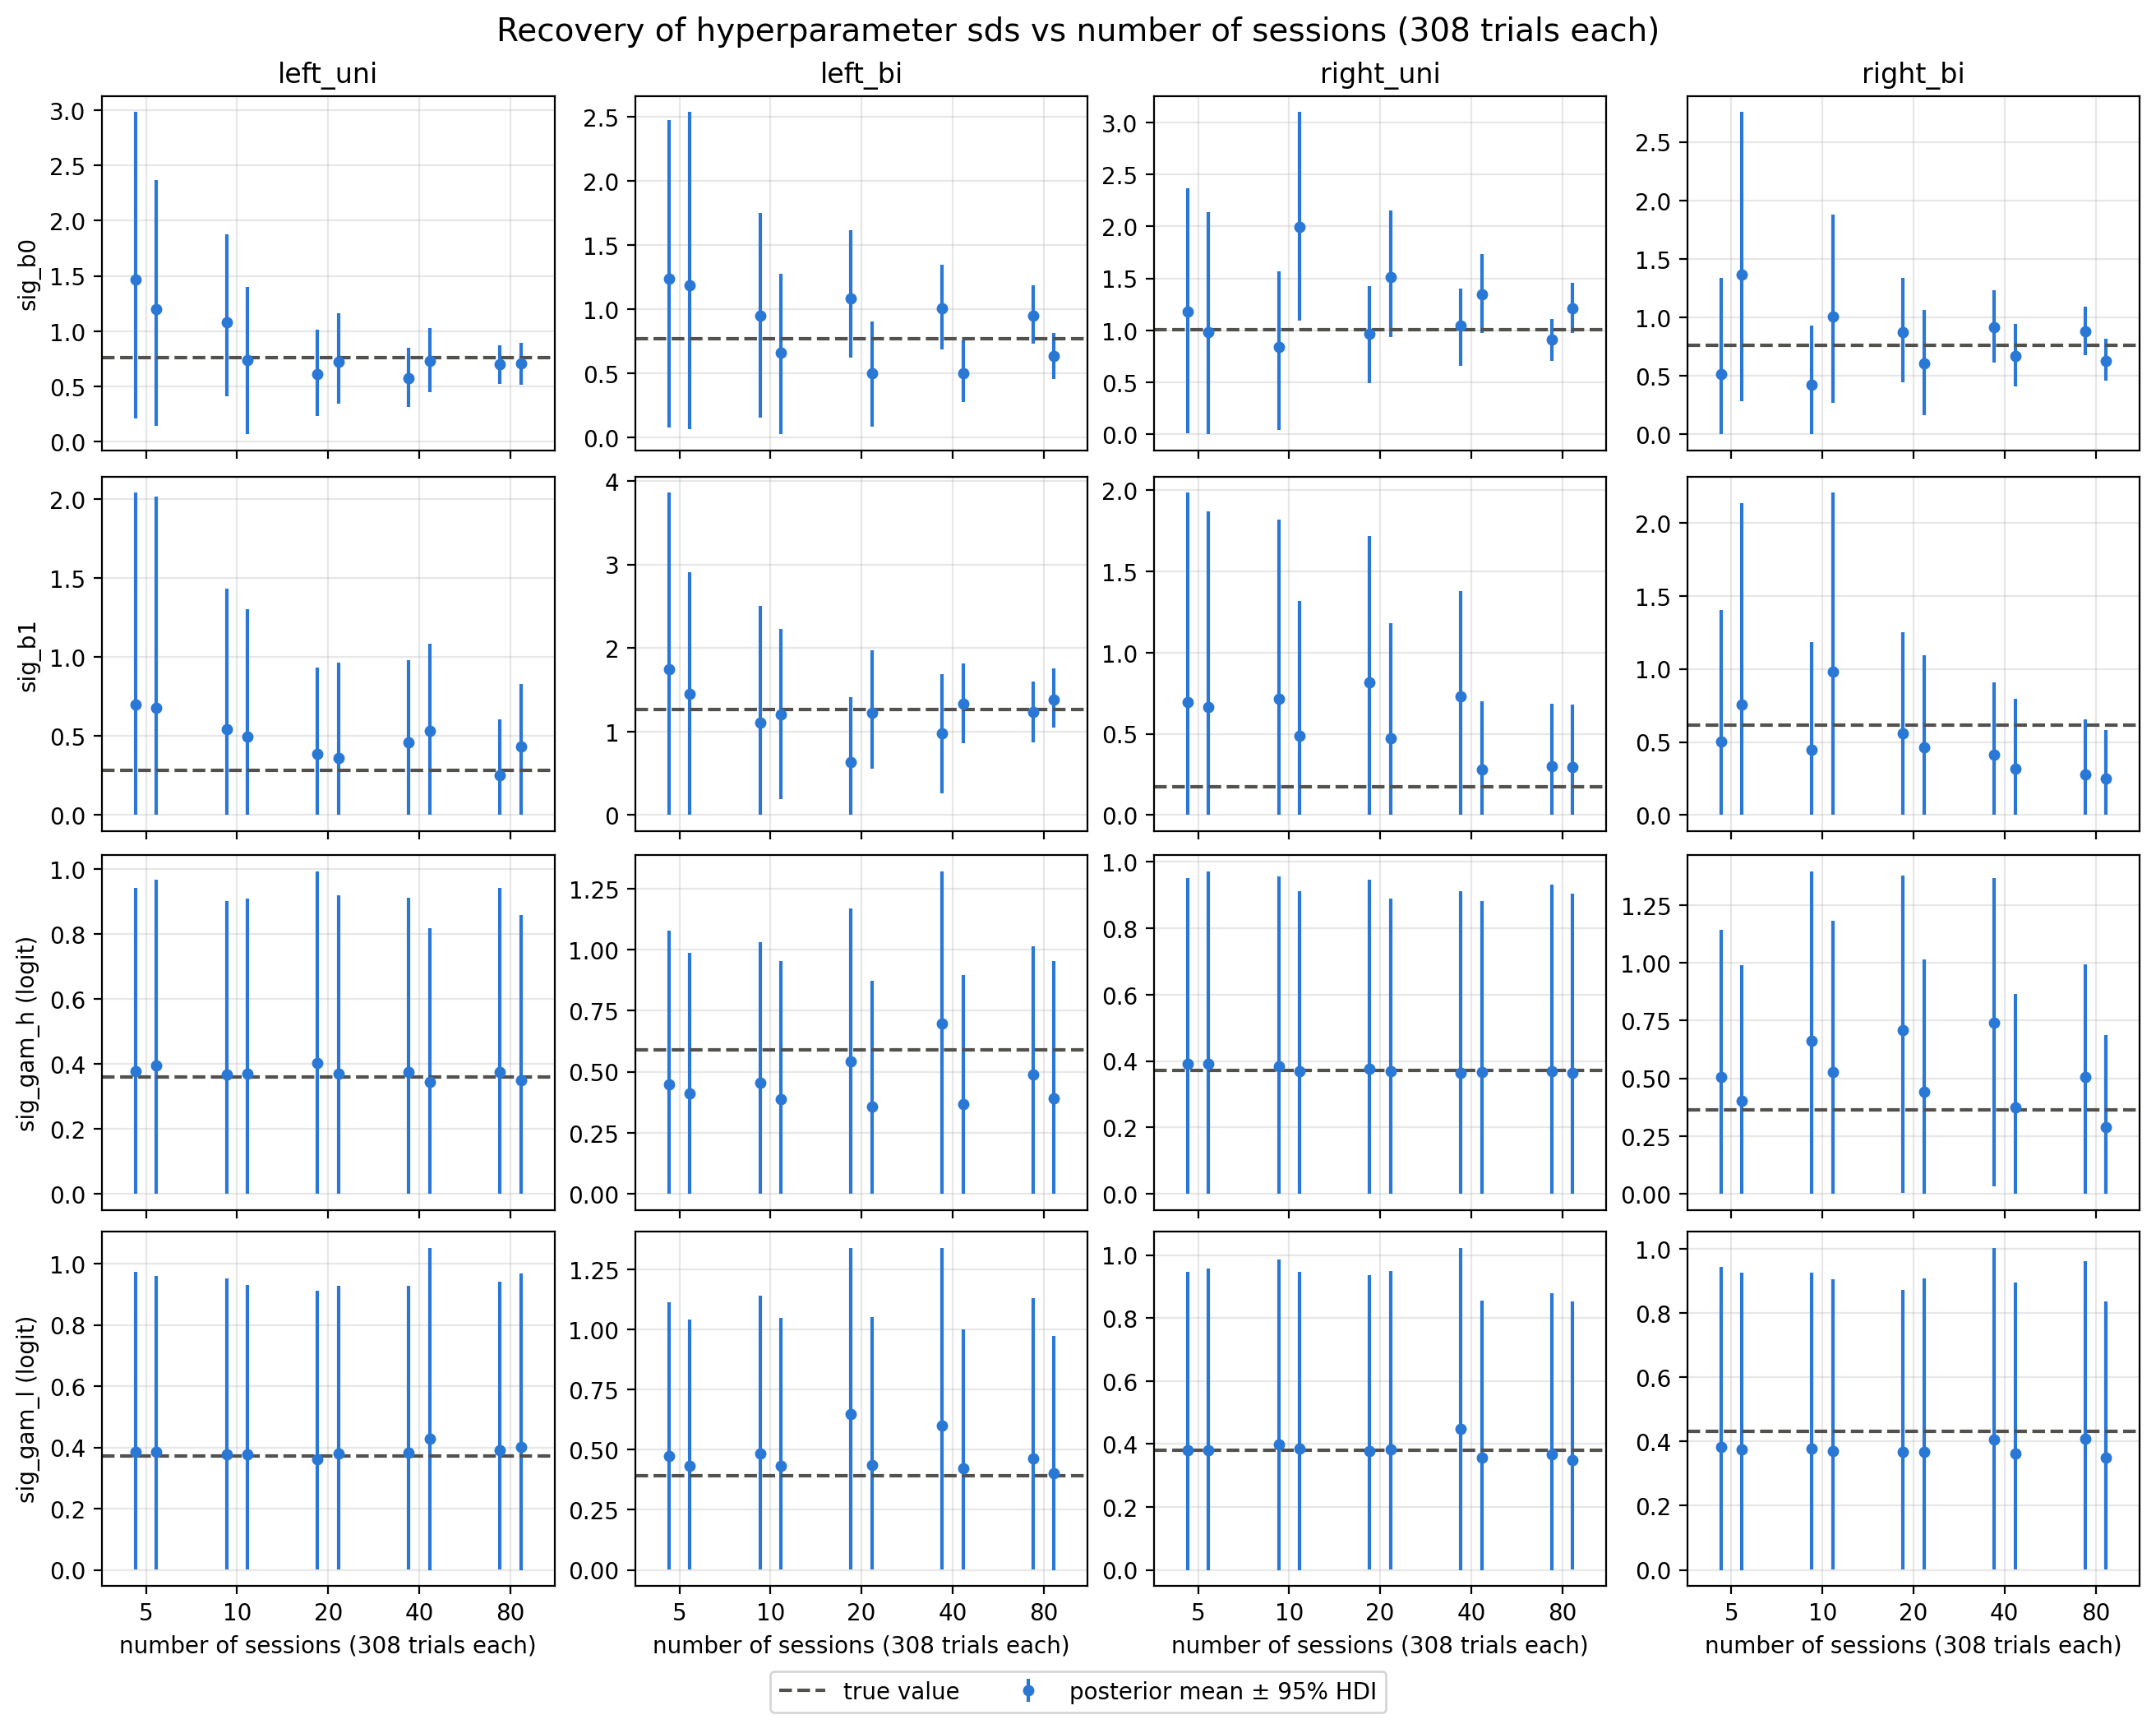
\includegraphics[width=\textwidth]{hyper_sds_recovery_vs_sessions.png}
\caption{Posterior mean and 95\% HDI of the between-session standard deviations
against the number of sessions.}
\label{fig:sds_sessions}
\end{figure}

\begin{table}[H]
\centering
\caption{Between-session sds at 80 sessions: true value and posterior mean
[95\% HDI], averaged over replicates.}
\label{tab:sds80}
\resizebox{\textwidth}{!}{%
\begin{tabular}{lcccc}
\toprule
 & left\_uni & left\_bi & right\_uni & right\_bi \\
\midrule
$\sigma_{\beta_0}$ true & 0.76 & 0.77 & 1.01 & 0.76 \\
\quad posterior & 0.70 [0.52, 0.88] & 0.79 [0.59, 1.00] & 1.06 [0.84, 1.29] & 0.75 [0.56, 0.95] \\
$\sigma_{\beta_1}$ true & 0.29 & 1.27 & 0.17 & 0.62 \\
\quad posterior & 0.34 [0.00, 0.72] & 1.31 [0.96, 1.68] & 0.30 [0.00, 0.68] & 0.26 [0.00, 0.62] \\
$\sigma_{\gamma_h}$ true & 0.36 & 0.59 & 0.37 & 0.36 \\
\quad posterior & 0.36 [0.00, 0.90] & 0.44 [0.00, 0.99] & 0.37 [0.00, 0.92] & 0.40 [0.00, 0.84] \\
$\sigma_{\gamma_l}$ true & 0.37 & 0.39 & 0.38 & 0.43 \\
\quad posterior & 0.40 [0.00, 0.96] & 0.43 [0.00, 1.05] & 0.36 [0.00, 0.86] & 0.38 [0.00, 0.90] \\
\bottomrule
\end{tabular}}
\end{table}

\paragraph{$\sigma_{\beta_0}$:} Recovered at 80 sessions in every group
(Table~\ref{tab:sds80}). With fewer sessions it can be well off: for right\_uni the
posterior mean is 1.42, 1.24 and 1.19 at 10, 20 and 40 sessions against a true 1.01.

\paragraph{$\sigma_{\beta_1}$:} Recovered when it is large: for left\_bi (true 1.27) the
posterior is 1.31 [0.96, 1.68] at 80 sessions. The smaller values (0.17--0.62) cannot be
told apart from 0 at these data sizes: their HDIs start at 0, and for right\_bi the
posterior mean falls to 0.26 at 80 sessions against a true 0.62, with the HDI just
reaching the truth.

\paragraph{$\sigma_{\gamma_h}$, $\sigma_{\gamma_l}$:} Not identified. Their posterior
means are 0.35--0.59 in every fit, their HDIs start at 0 and end at 0.84--1.29, and they
barely change with the amount of data: they reflect the prior (mean 0.40, 95\% point
0.98). The true values (0.36--0.59) happen to lie near the prior median (0.34), so
the 100\% coverage says little.

\subsection{Session-level parameters}
\label{sec:session}

\begin{figure}[H]
\centering
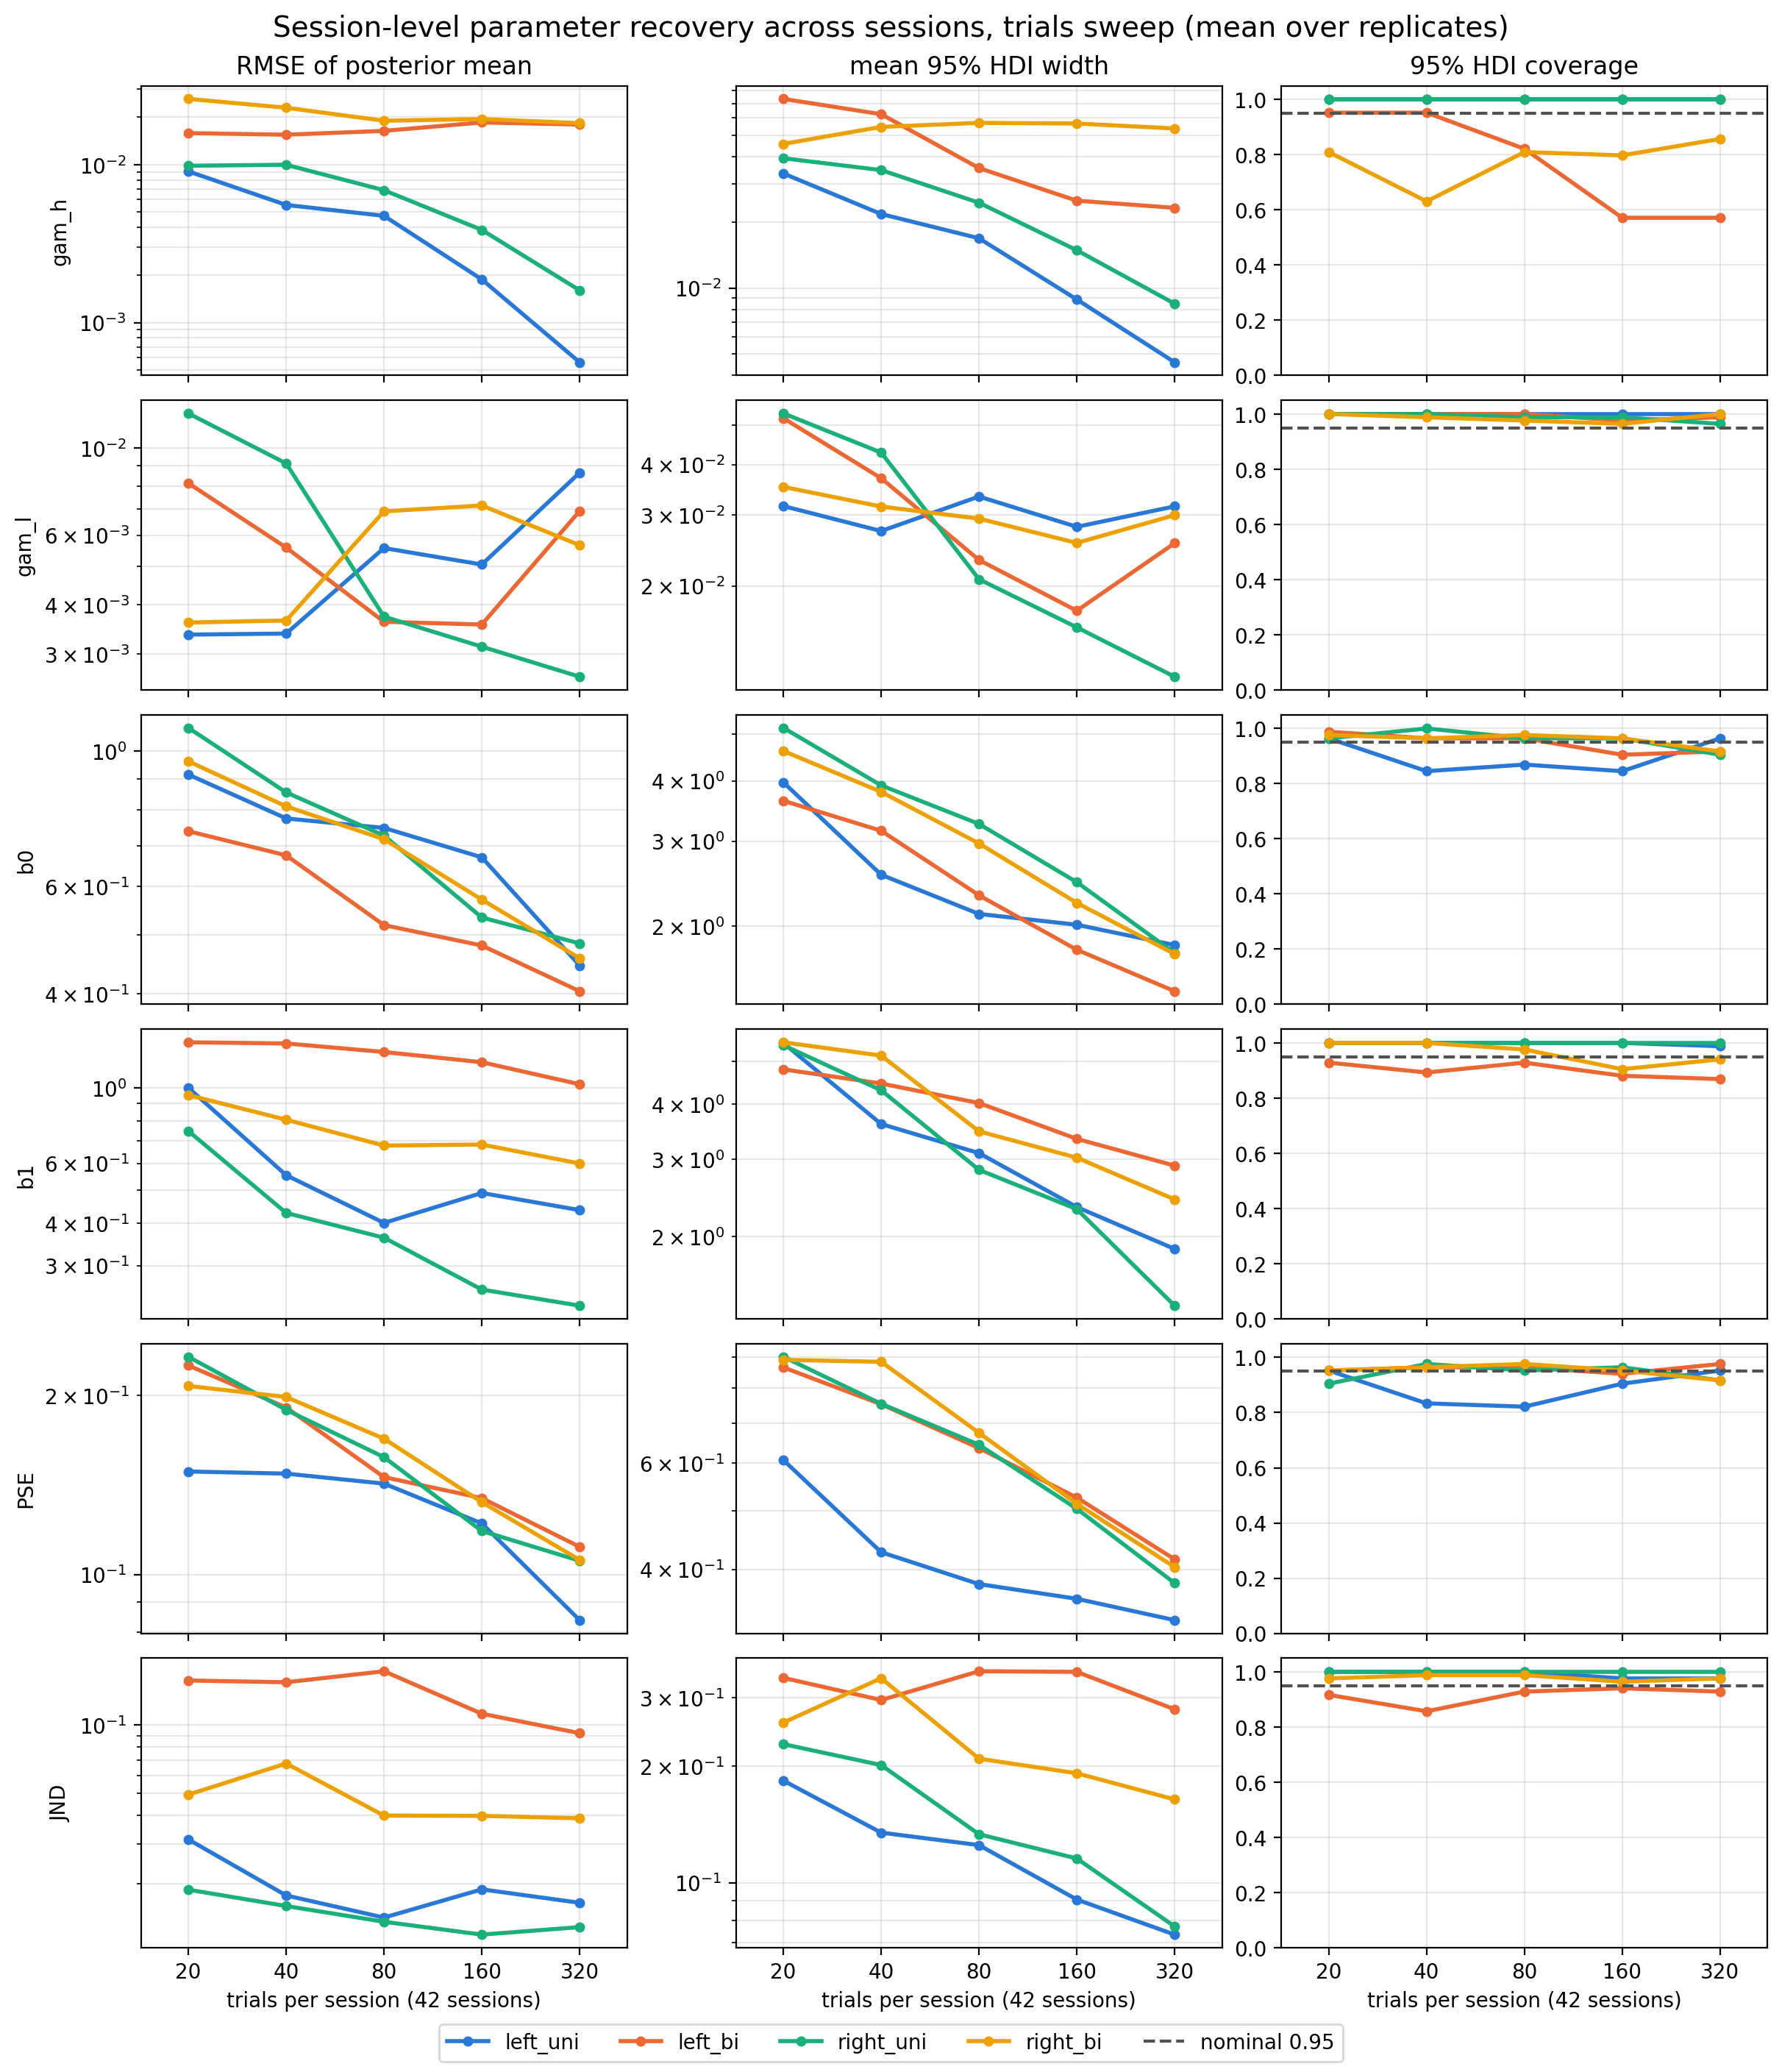
\includegraphics[width=0.92\textwidth]{session_params_error_width_coverage_vs_trials.png}
\caption{Session-level recovery against trials per session (42 sessions),
averaged over replicates. Left: RMSE of the posterior mean across sessions.
Middle: mean 95\% HDI width. Right: fraction of sessions whose HDI contains the
true value.}
\label{fig:session_trials}
\end{figure}

\begin{figure}[H]
\centering
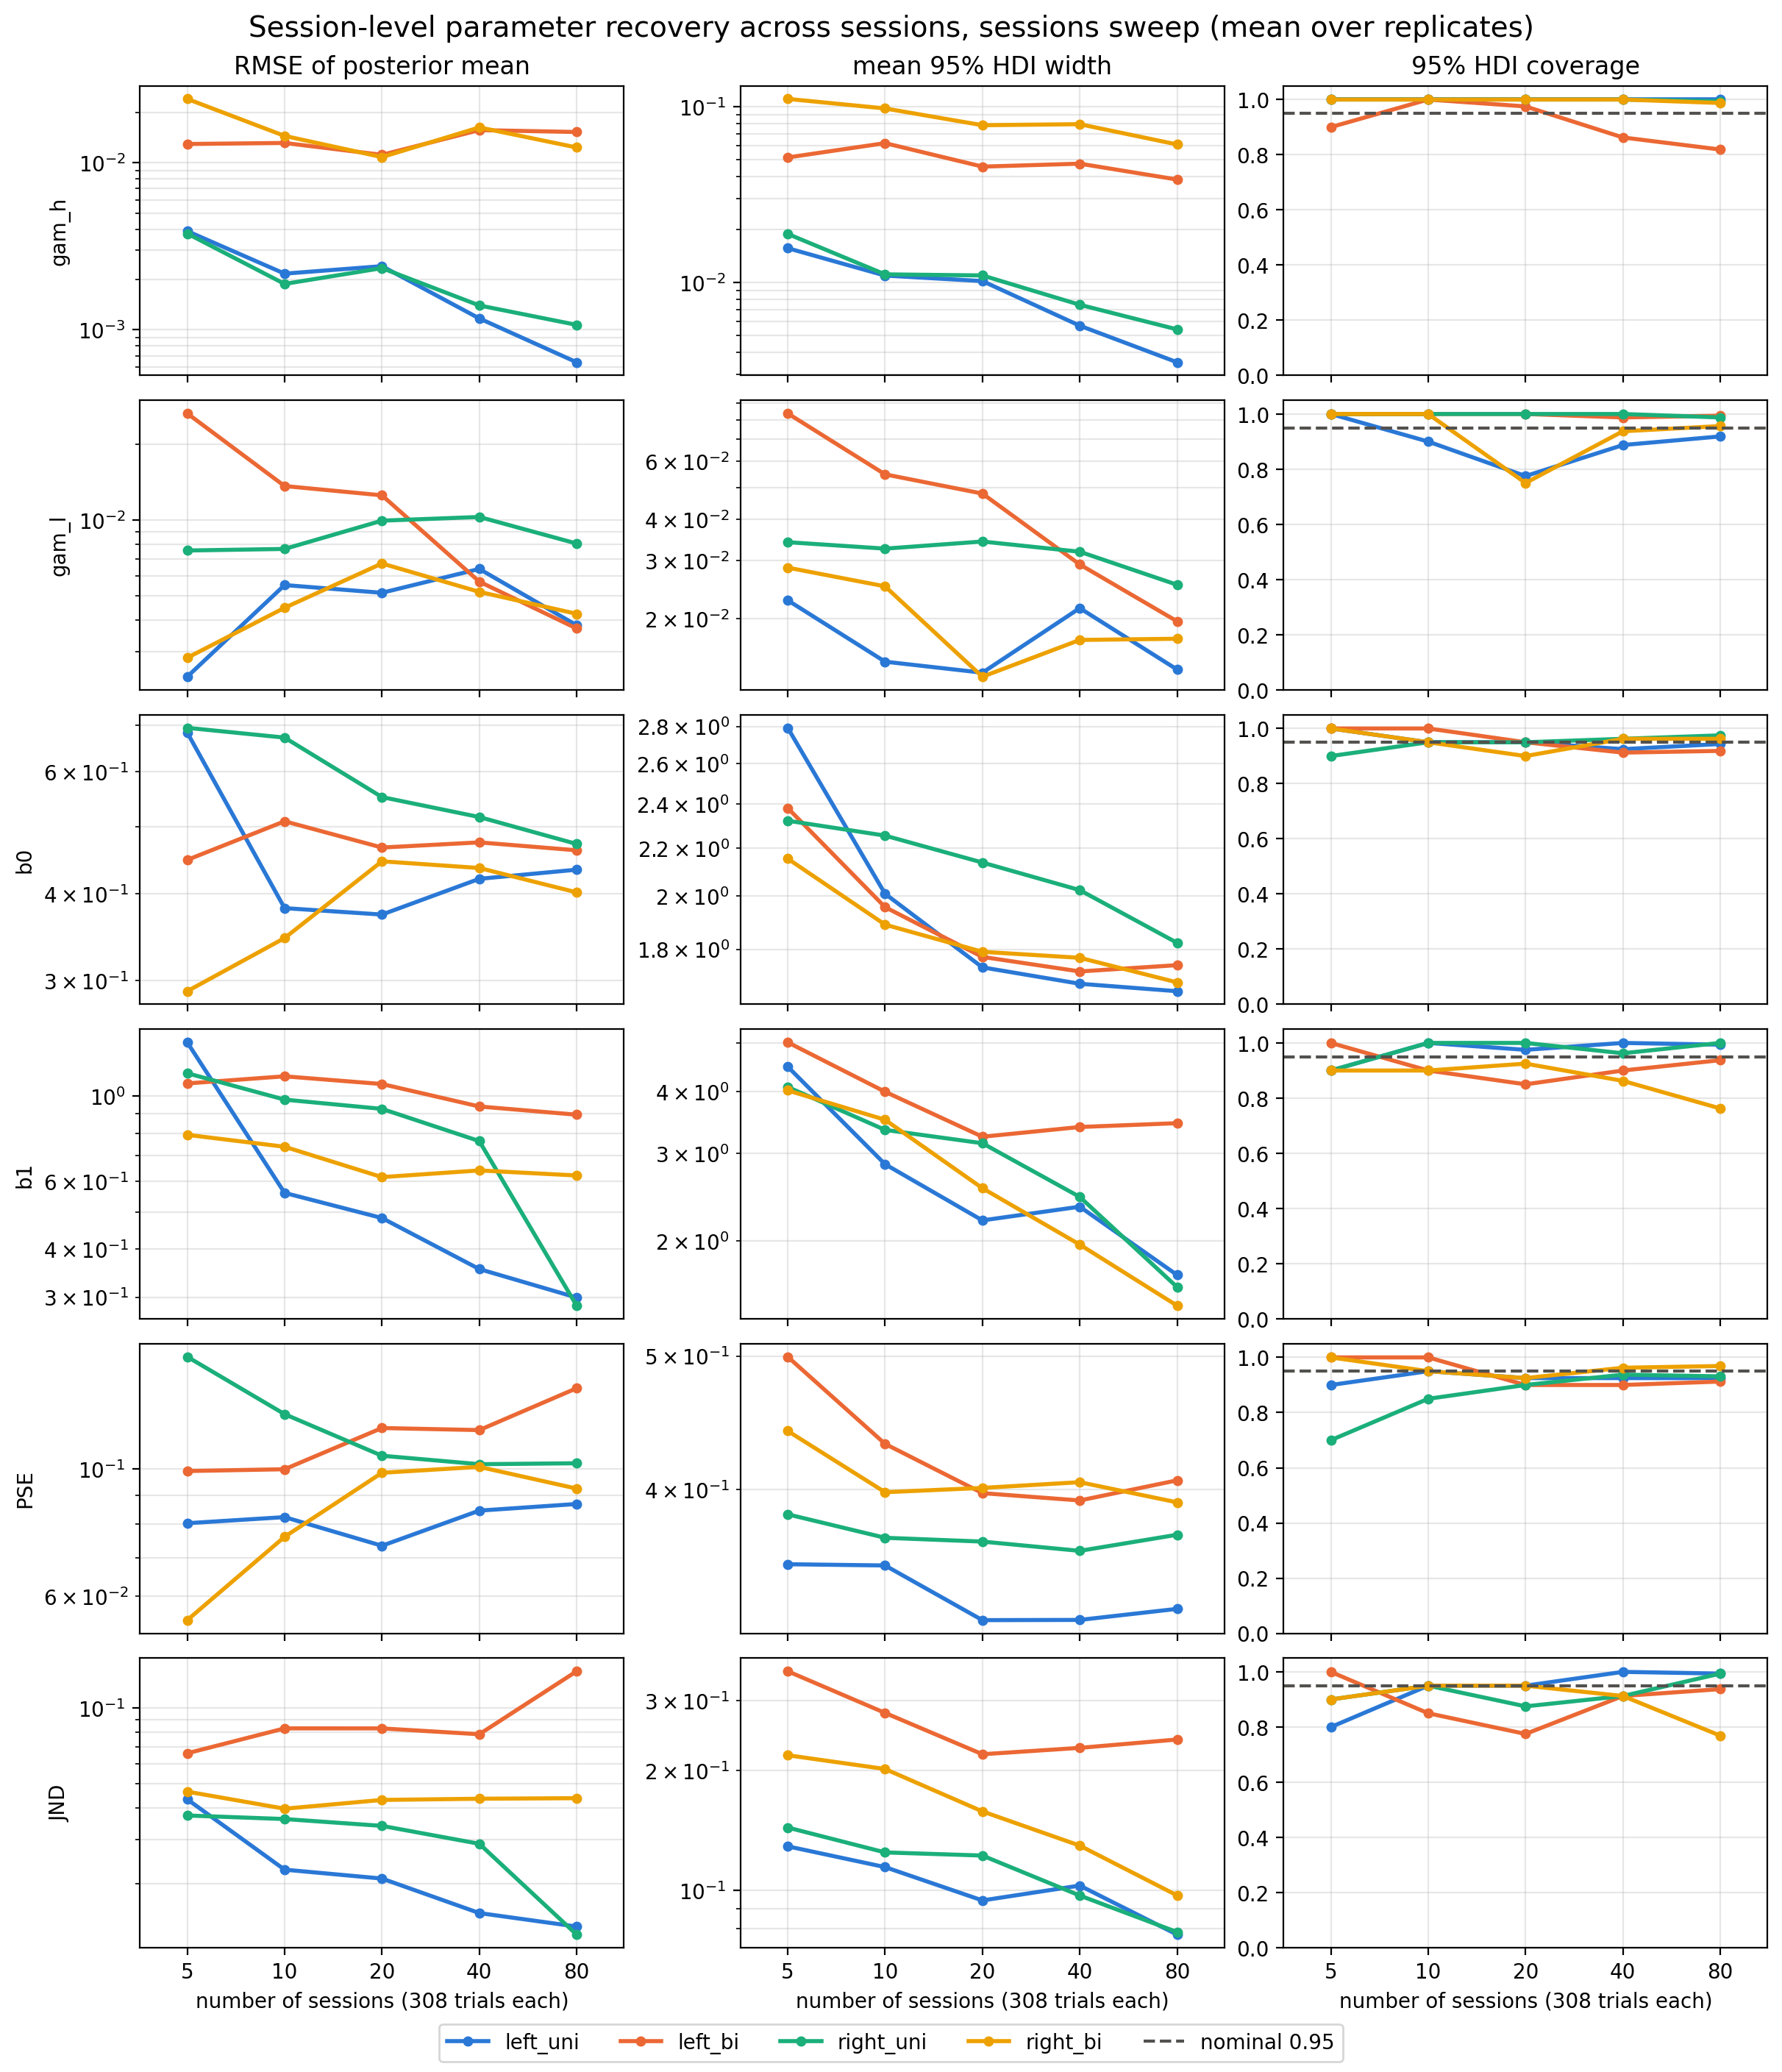
\includegraphics[width=0.92\textwidth]{session_params_error_width_coverage_vs_sessions.png}
\caption{As Figure~\ref{fig:session_trials}, against the number of sessions
(308 trials each).}
\label{fig:session_sessions}
\end{figure}

\begin{table}[H]
\centering
\caption{Session-level recovery at 320 trials per session (42 sessions, both
replicates): RMSE of the posterior mean / mean HDI width / coverage. PSE and JND in
standardized units (1 unit = 14.63 $\mu m$).}
\label{tab:session320}
\begin{tabular}{lcccc}
\toprule
 & left\_uni & left\_bi & right\_uni & right\_bi \\
\midrule
PSE & 0.08 / 0.33 / 0.95 & 0.11 / 0.42 / 0.98 & 0.11 / 0.38 / 0.92 & 0.11 / 0.40 / 0.92 \\
JND & 0.017 / 0.07 / 0.98 & 0.095 / 0.28 / 0.93 & 0.013 / 0.08 / 1.00 & 0.039 / 0.16 / 0.98 \\
$\beta_0$ & 0.45 / 1.83 / 0.96 & 0.40 / 1.47 / 0.92 & 0.49 / 1.76 / 0.90 & 0.46 / 1.75 / 0.92 \\
$\beta_1$ & 0.44 / 1.88 / 0.99 & 1.02 / 2.90 / 0.87 & 0.23 / 1.39 / 1.00 & 0.60 / 2.43 / 0.94 \\
$\gamma_h$ & 0.001 / 0.005 / 1.00 & 0.018 / 0.023 / 0.57 & 0.002 / 0.008 / 1.00 & 0.018 / 0.054 / 0.86 \\
$\gamma_l$ & 0.009 / 0.031 / 1.00 & 0.008 / 0.026 / 0.99 & 0.003 / 0.012 / 0.96 & 0.006 / 0.030 / 1.00 \\
\bottomrule
\end{tabular}
\end{table}

\paragraph{PSE and JND.} The per-session PSEs are recovered well: at 320 trials the
RMSE is 0.08--0.11 standardized units (1.2--1.6 $\mu m$) and the coverage 0.92--0.98
(Table~\ref{tab:session320}), down from an RMSE of 0.15--0.23 at 20 trials. The JND
is recovered with an RMSE of 0.013--0.039 in three groups. For left\_bi, whose sessions
differ strongly in slope ($\sigma_{\beta_1} = 1.27$, true session JNDs from 2.4 to
15.9 $\mu m$), the RMSE is 0.095 (1.4 $\mu m$), with coverage 0.93.

\paragraph{$\beta_0$, $\beta_1$.} The individual coefficients are less precise than the
PSE and JND computed from them (HDI widths 1.4--2.9 at 320 trials). Coverage is 0.90--1.00,
except for the left\_bi slopes (0.87), the group with the largest slope spread.

\paragraph{Coverage.} With 84 sessions per group, the standard error of a coverage
estimate near 0.95 is about 0.024, so values of 0.90--0.92 are mildly low.

\paragraph{Lapse rates $\gamma_h$ and $\gamma_l$: a miss at the group level carries over
to every session.} With $\sigma_{\gamma_h}$ and $\sigma_{\gamma_l}$ not identified, the
session lapse rates are pulled strongly toward their group's typical value. The
session HDIs are therefore narrow (mean width 0.005--0.054), and when the group value
is off, every session of the group misses:
\begin{itemize}
  \item $\gamma_h$ of the bimanual groups is undercovered at 320 trials: 0.57 for
        left\_bi and 0.86 for right\_bi. In one replicate the left\_bi session
        posterior means average 0.005 against true values averaging 0.021 (coverage
        0.31), and the right\_bi ones 0.021 against 0.037 (coverage 0.71). In the other
        replicate right\_bi goes the other way (0.049 against 0.036).
  \item $\gamma_l$ of left\_uni is too high at 320 trials (posterior means averaging 0.016
        against 0.0085), the counterpart of the $\mu_{\gamma_l}$ error above; its HDIs
        still contain the truth.
\end{itemize}

\subsection{Posterior densities}

The following plots show the same fits as full posterior densities, darker for
larger datasets. They confirm the points above: the group means and $\sigma_{\beta_0}$
concentrate around the truth as data grow, while the posteriors of
$\sigma_{\gamma_h}$ and $\sigma_{\gamma_l}$ barely change.

\begin{figure}[H]
    \centering
    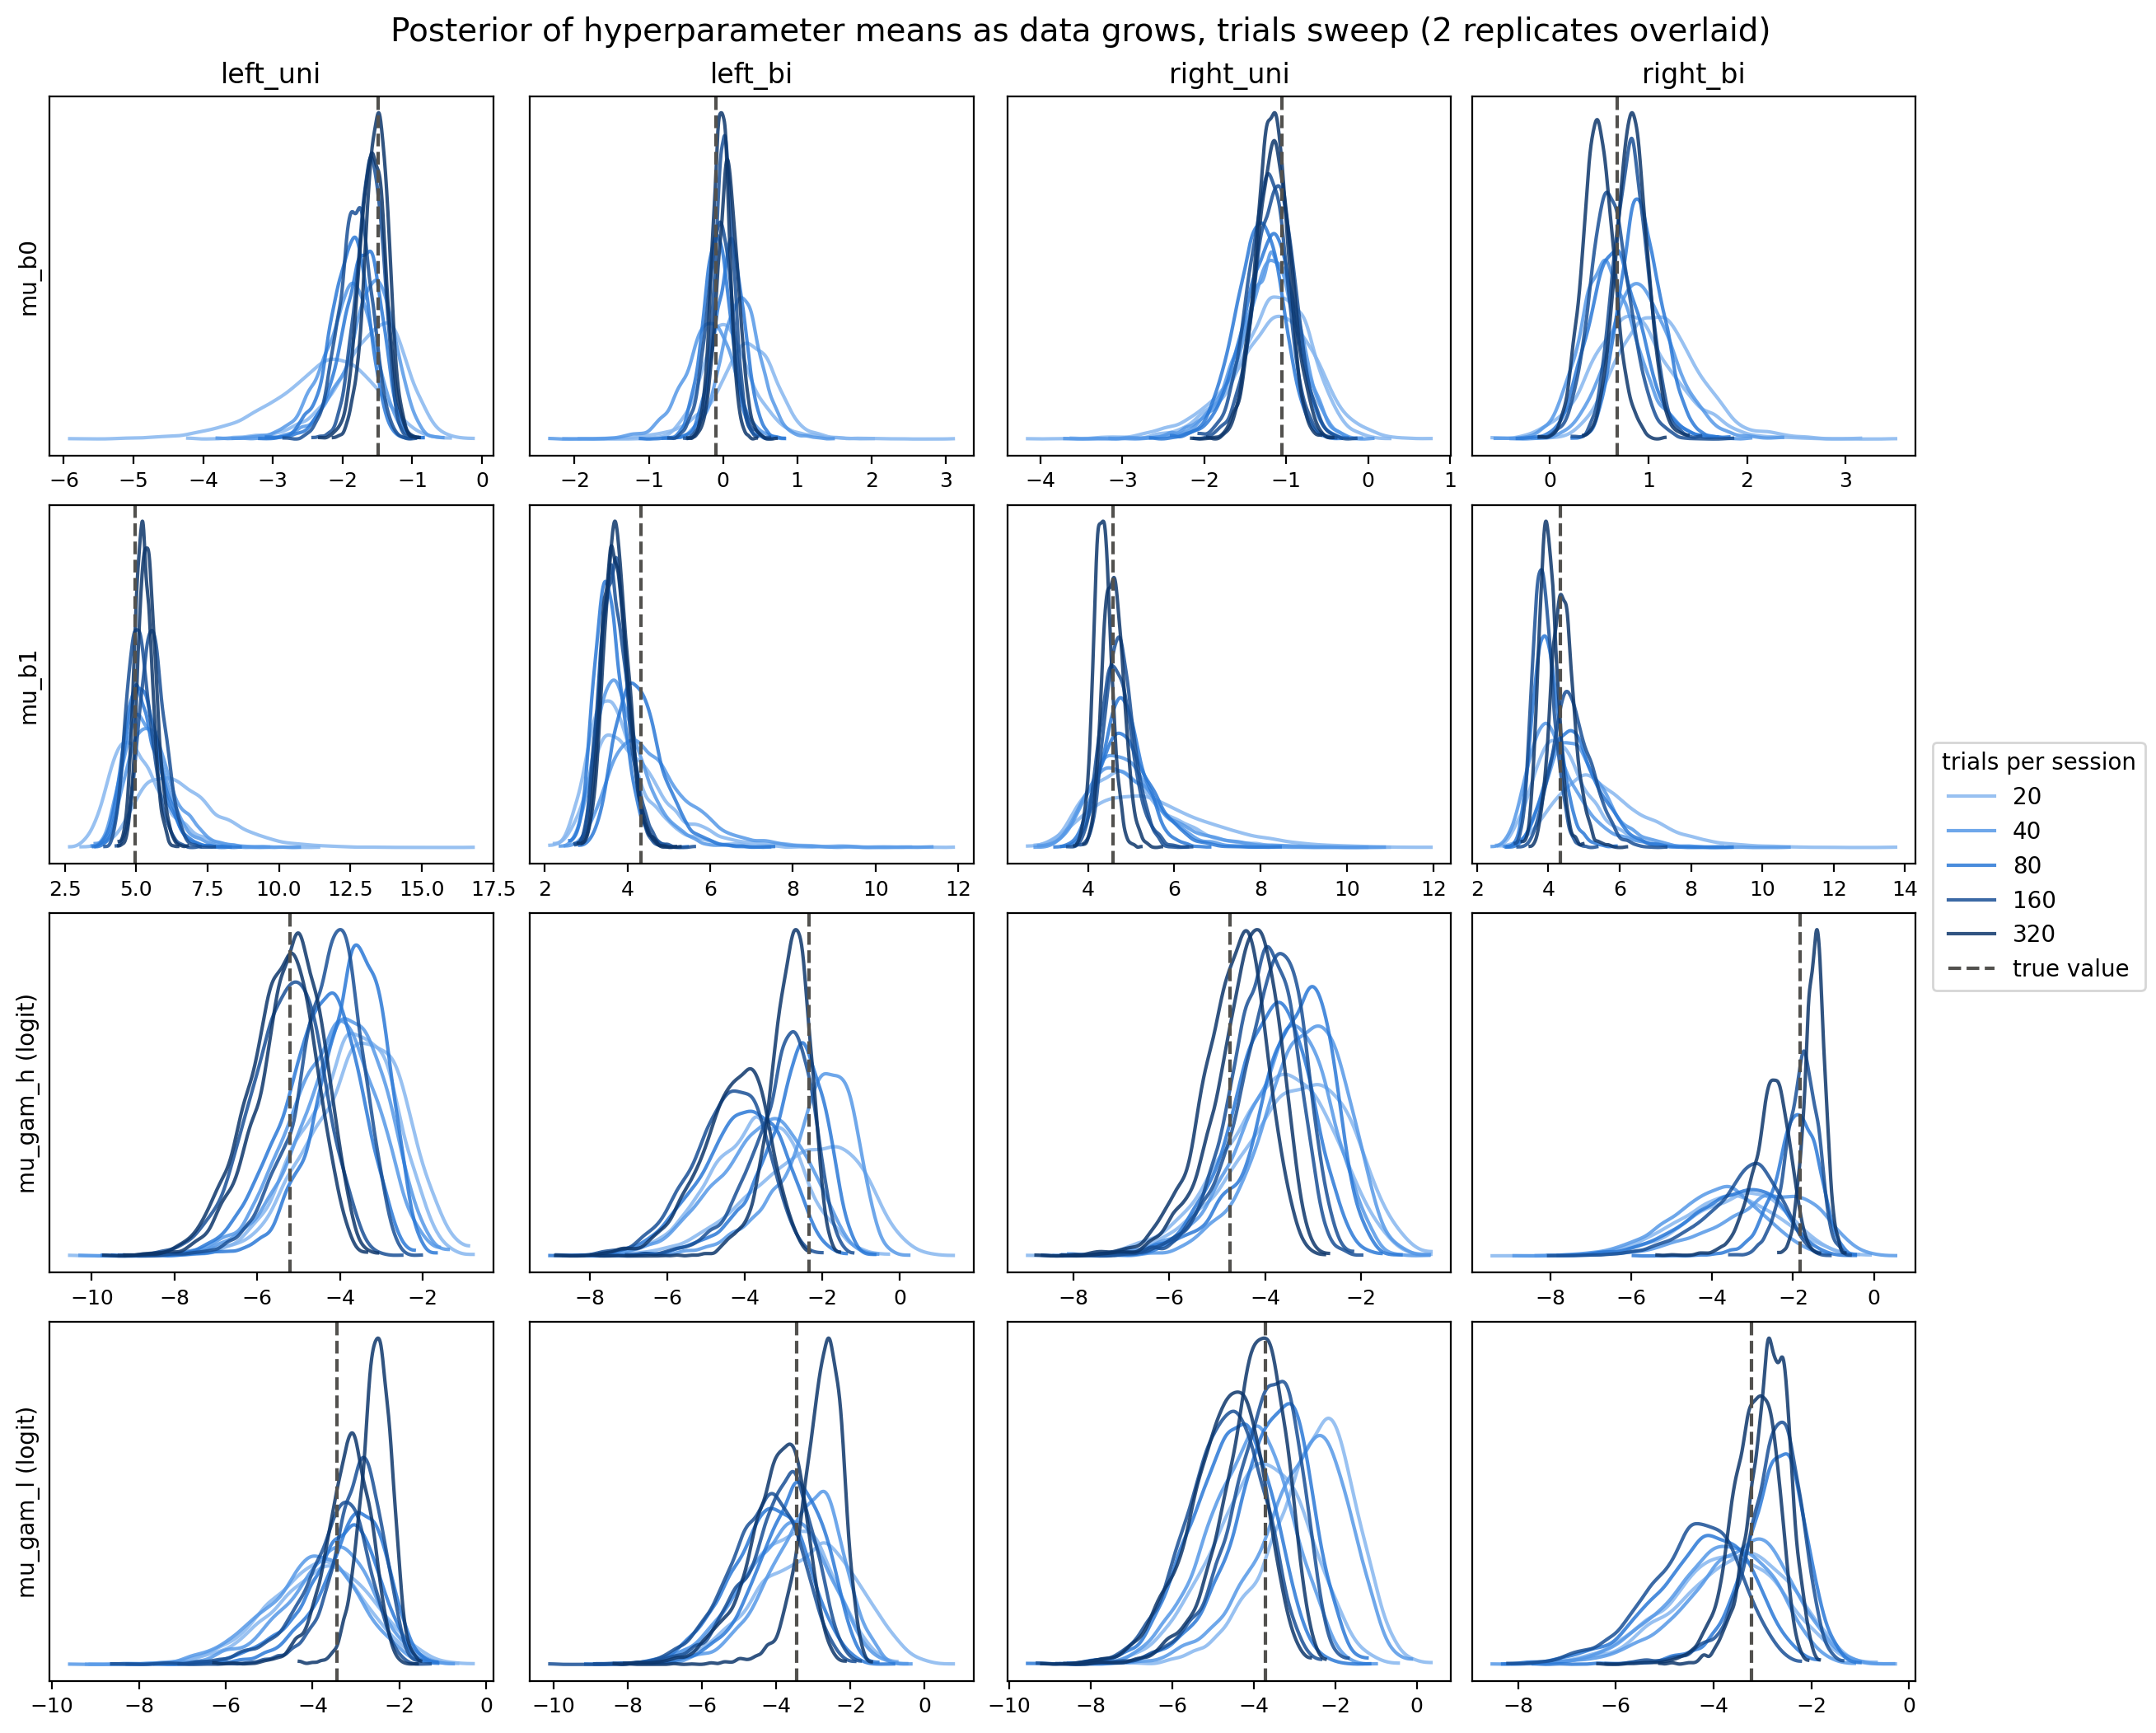
\includegraphics[width=1\linewidth]{hyper_means_density_vs_trials.png}
    \caption{Posteriors of mean hyperparameters as trials vary}
    \label{fig:means_density_trials}
\end{figure}

\begin{figure}[H]
    \centering
    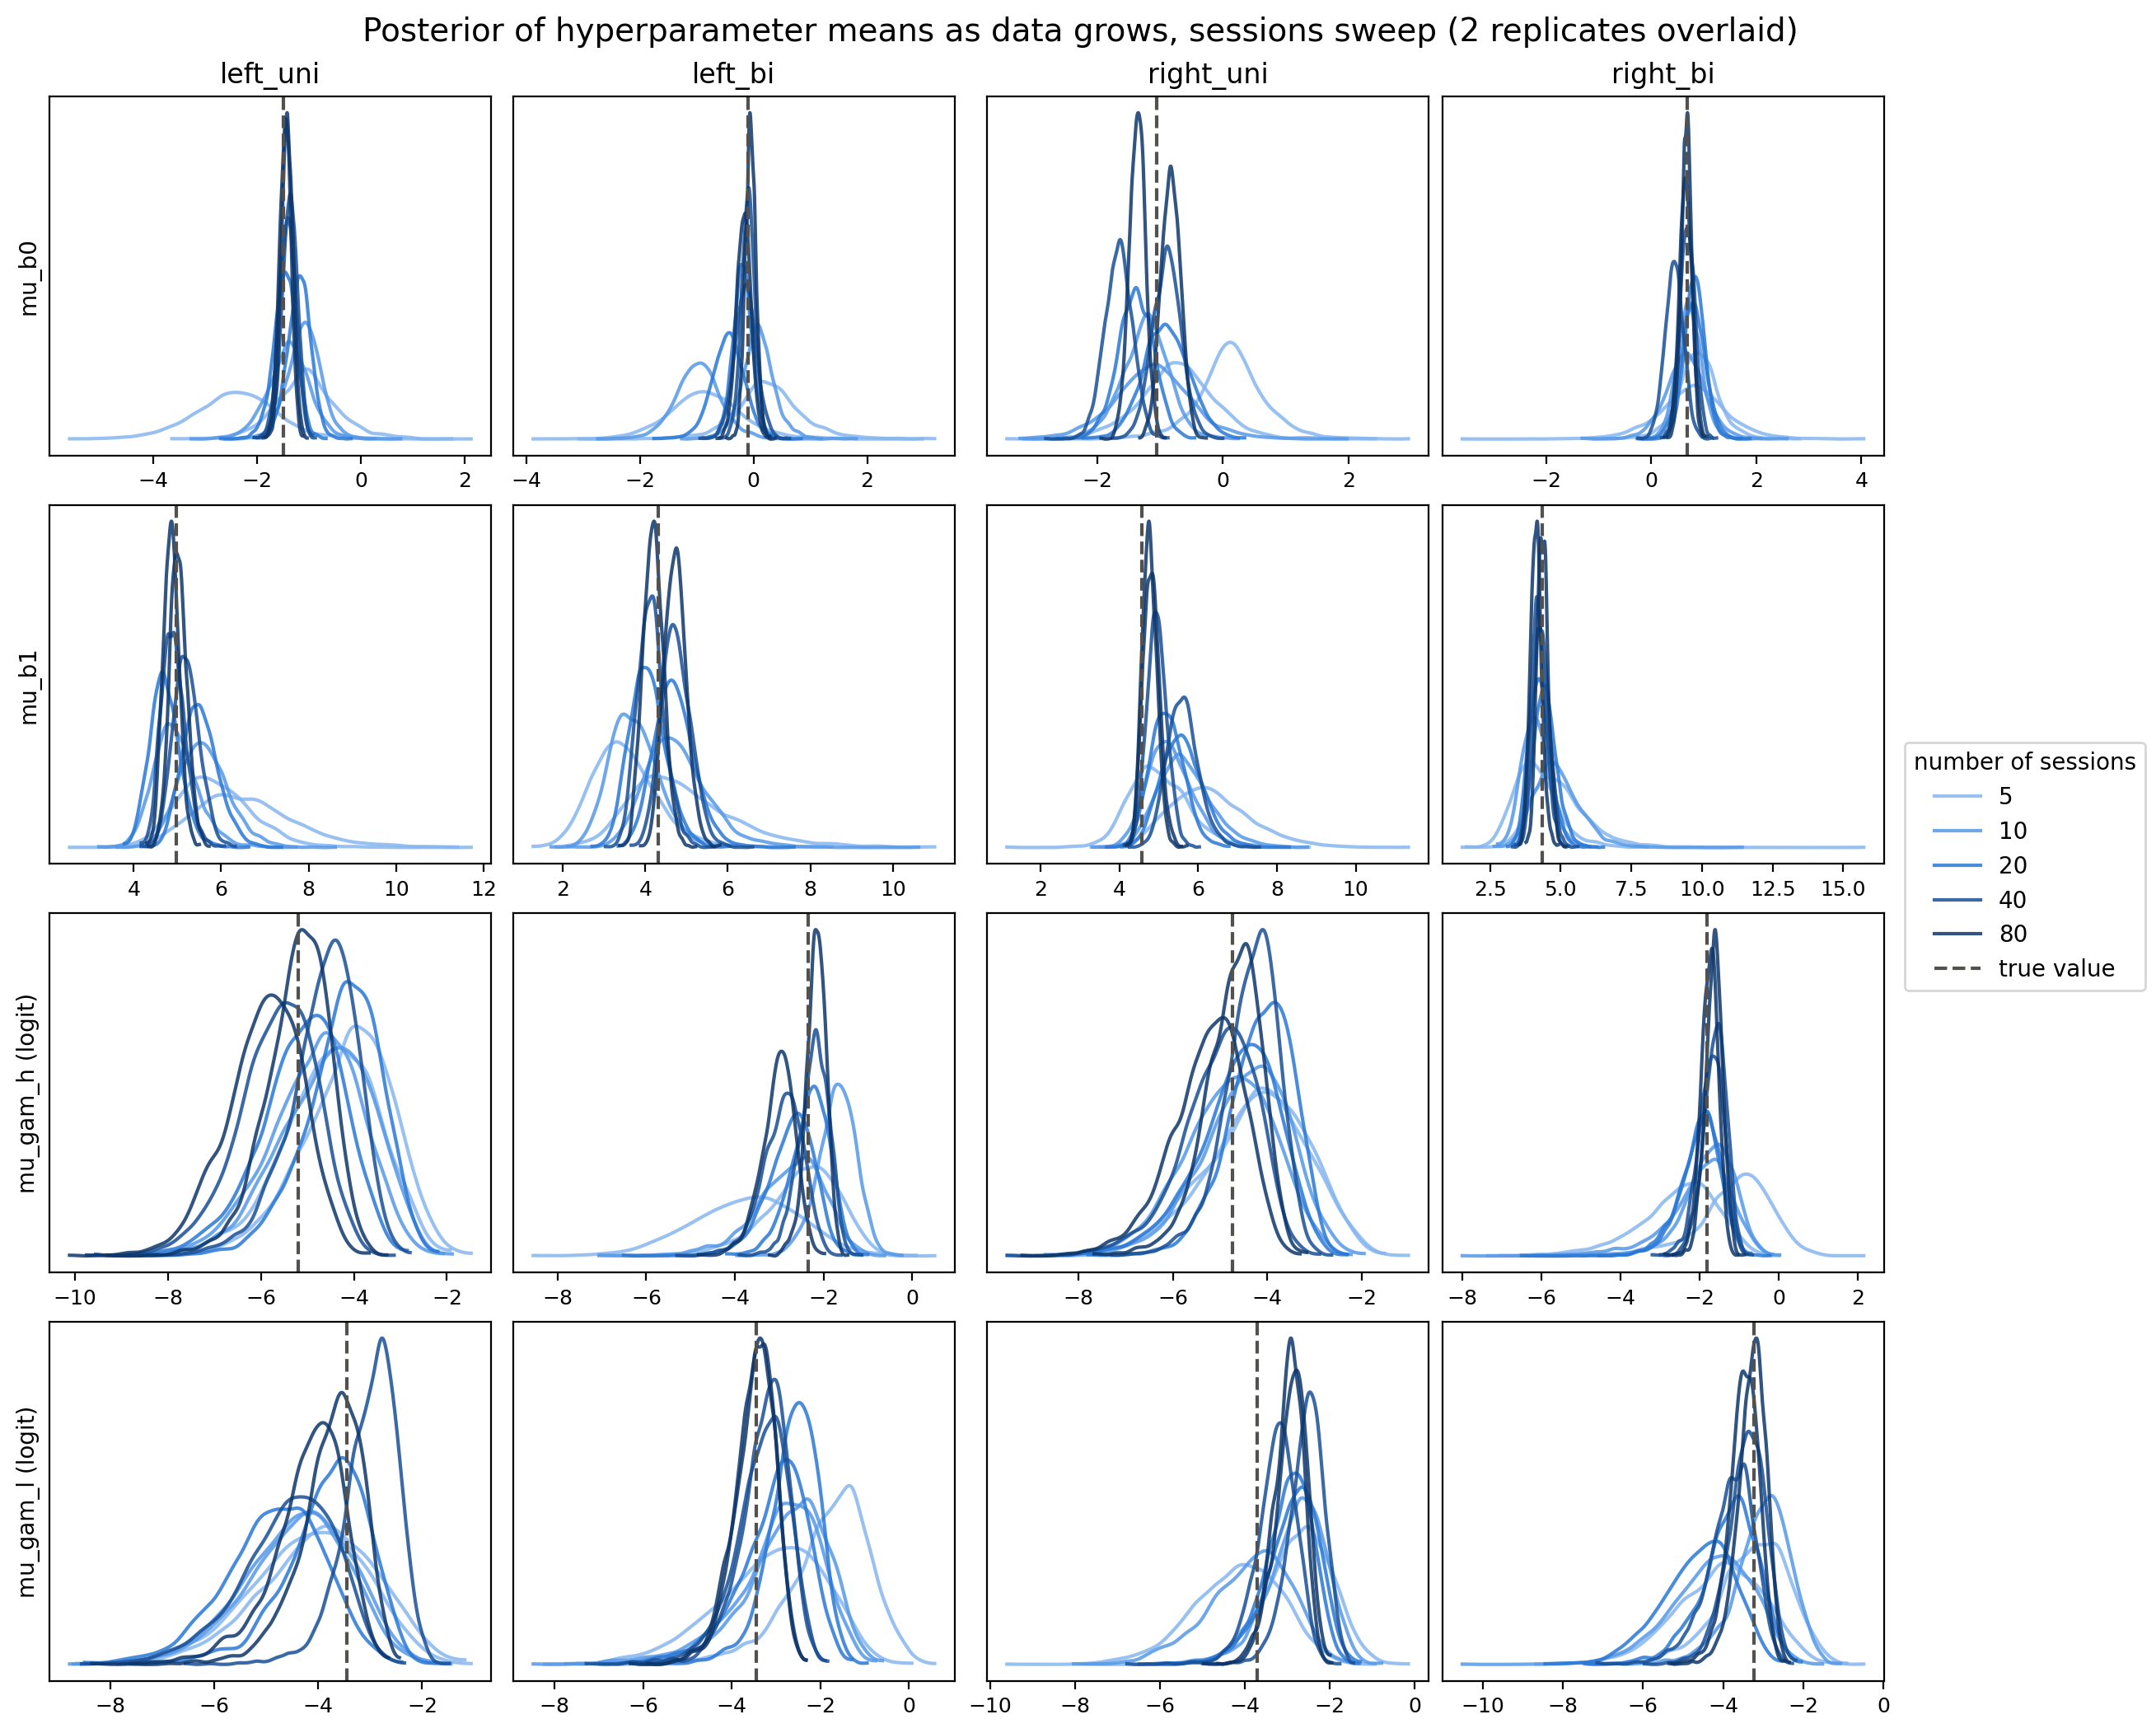
\includegraphics[width=1\linewidth]{hyper_means_density_vs_sessions.png}
    \caption{Posteriors of mean hyperparameters as sessions vary}
    \label{fig:means_density_sessions}
\end{figure}

\begin{figure}[H]
    \centering
    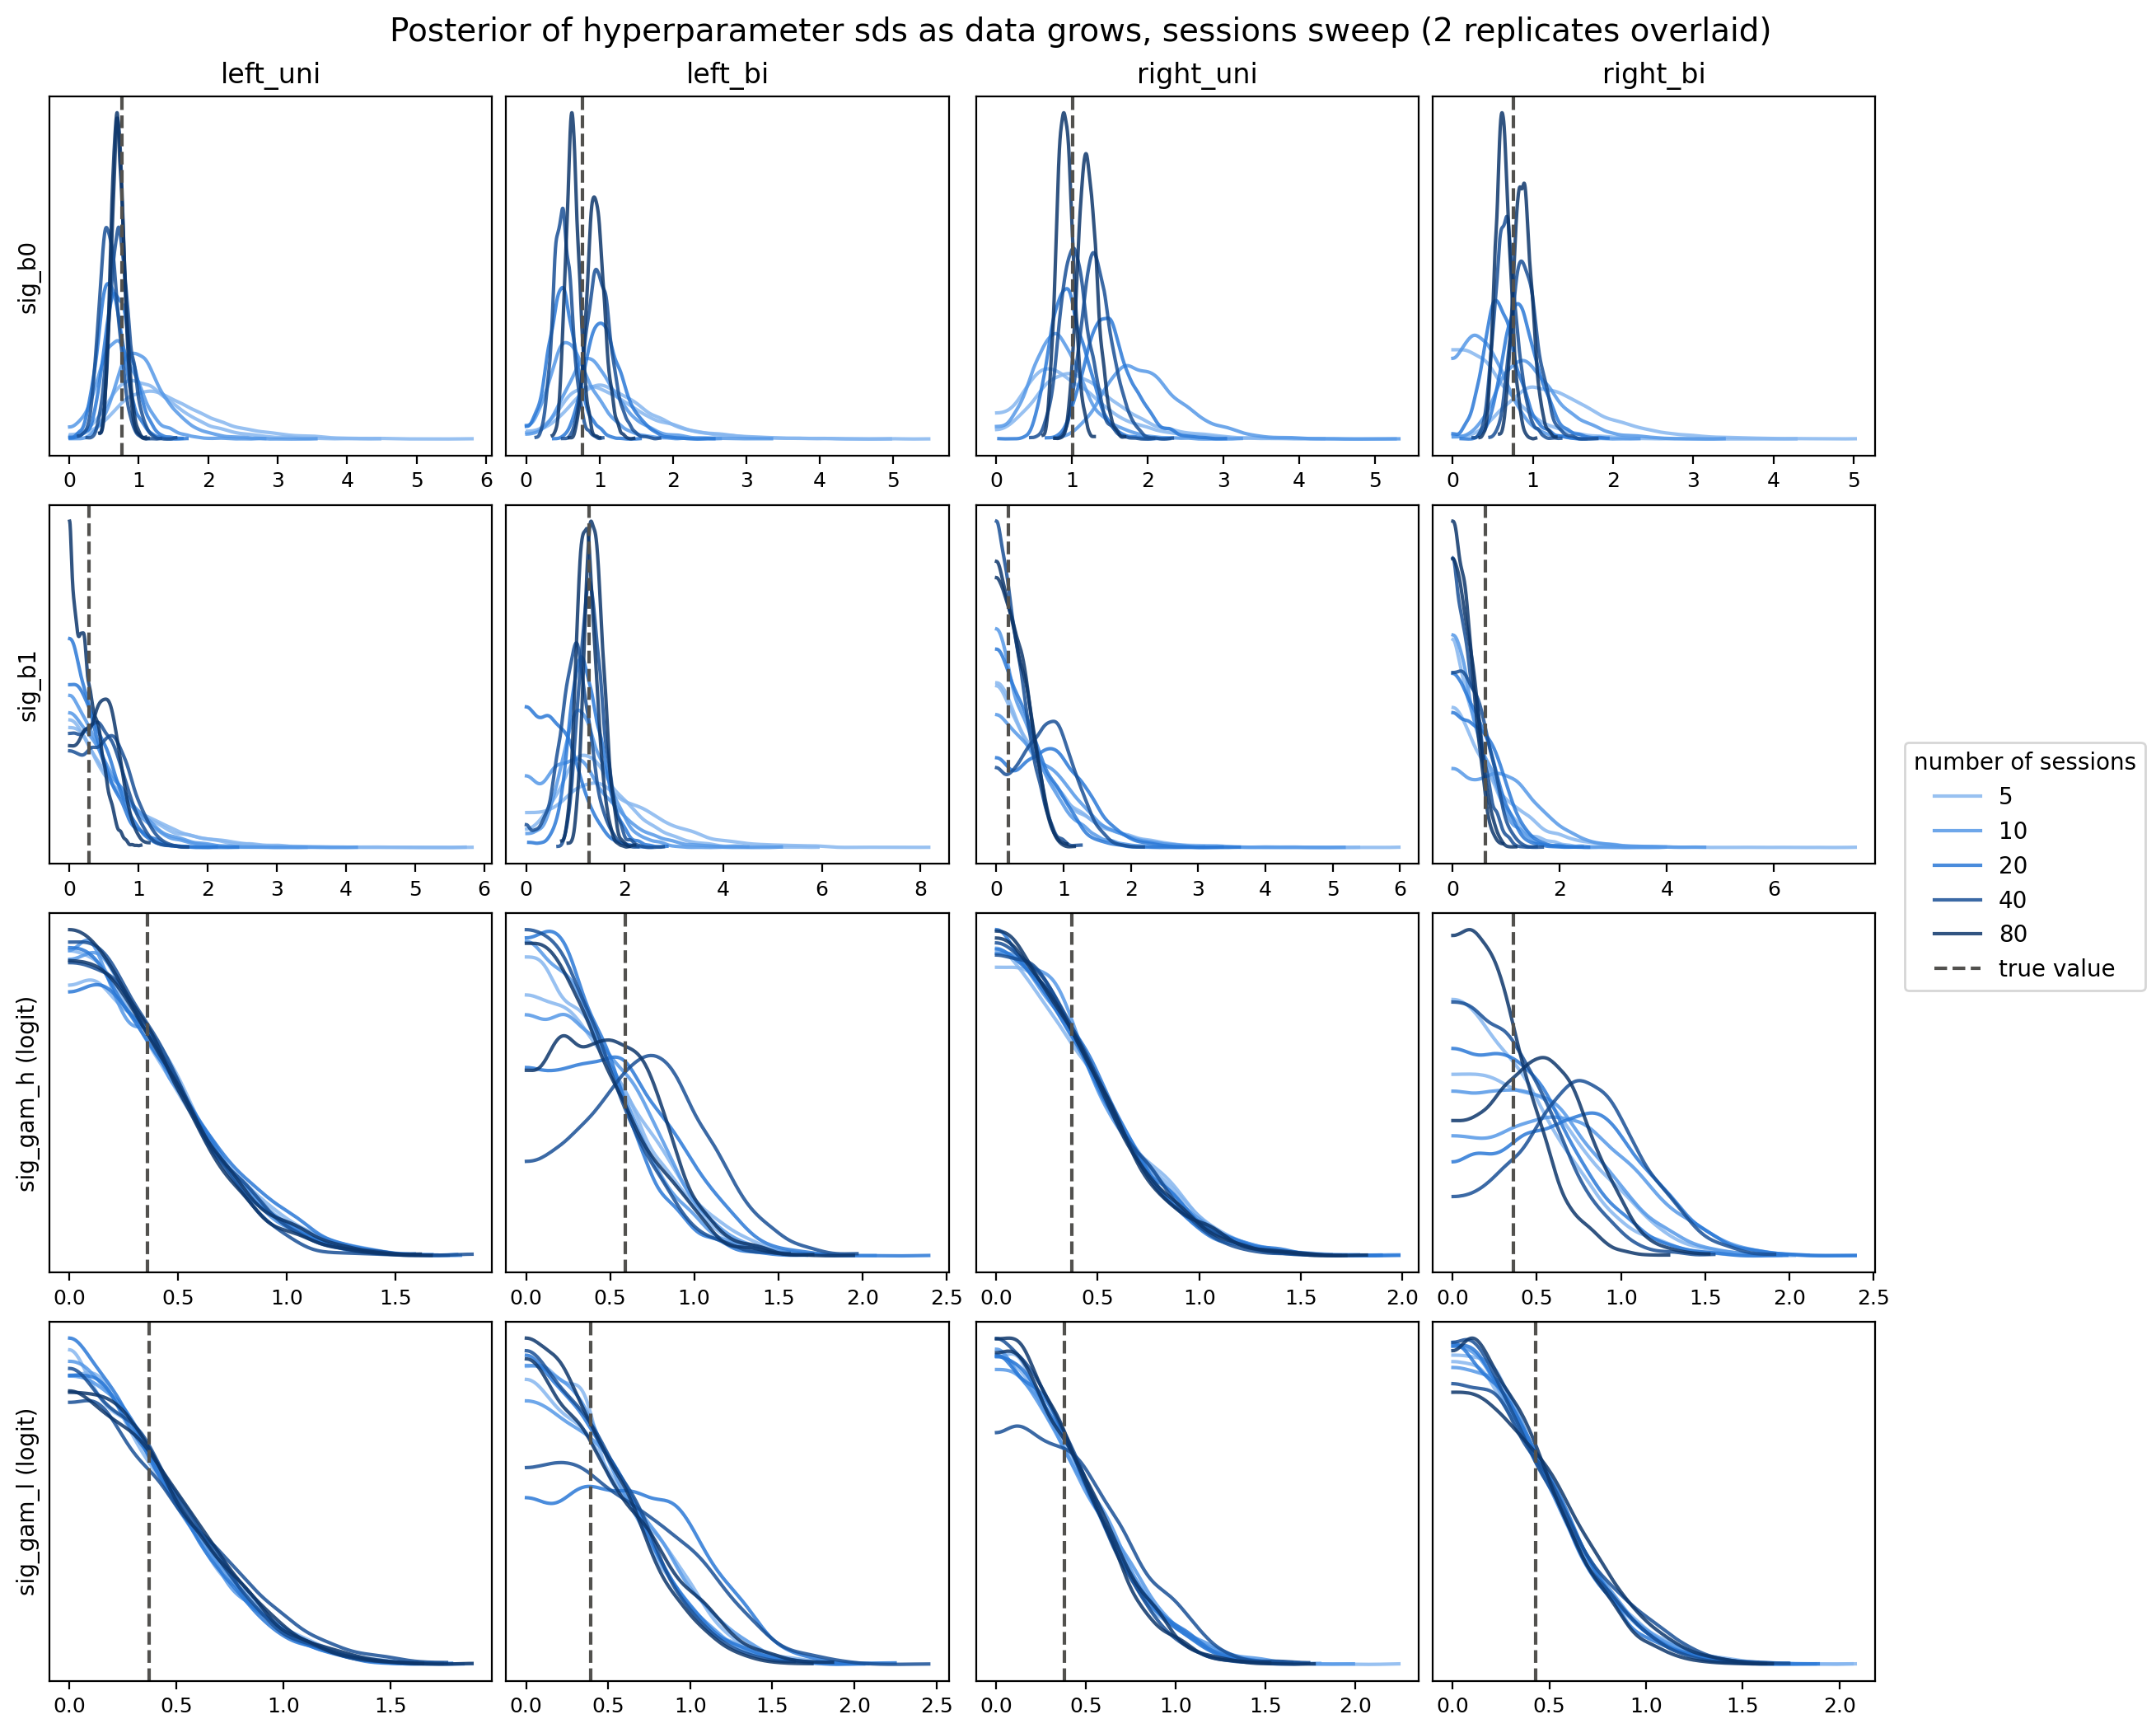
\includegraphics[width=1\linewidth]{hyper_sds_density_vs_sessions.png}
    \caption{Posteriors of sd hyperparameters as sessions vary}
    \label{fig:sds_density_sessions}
\end{figure}
\begin{figure}[H]
    \centering
    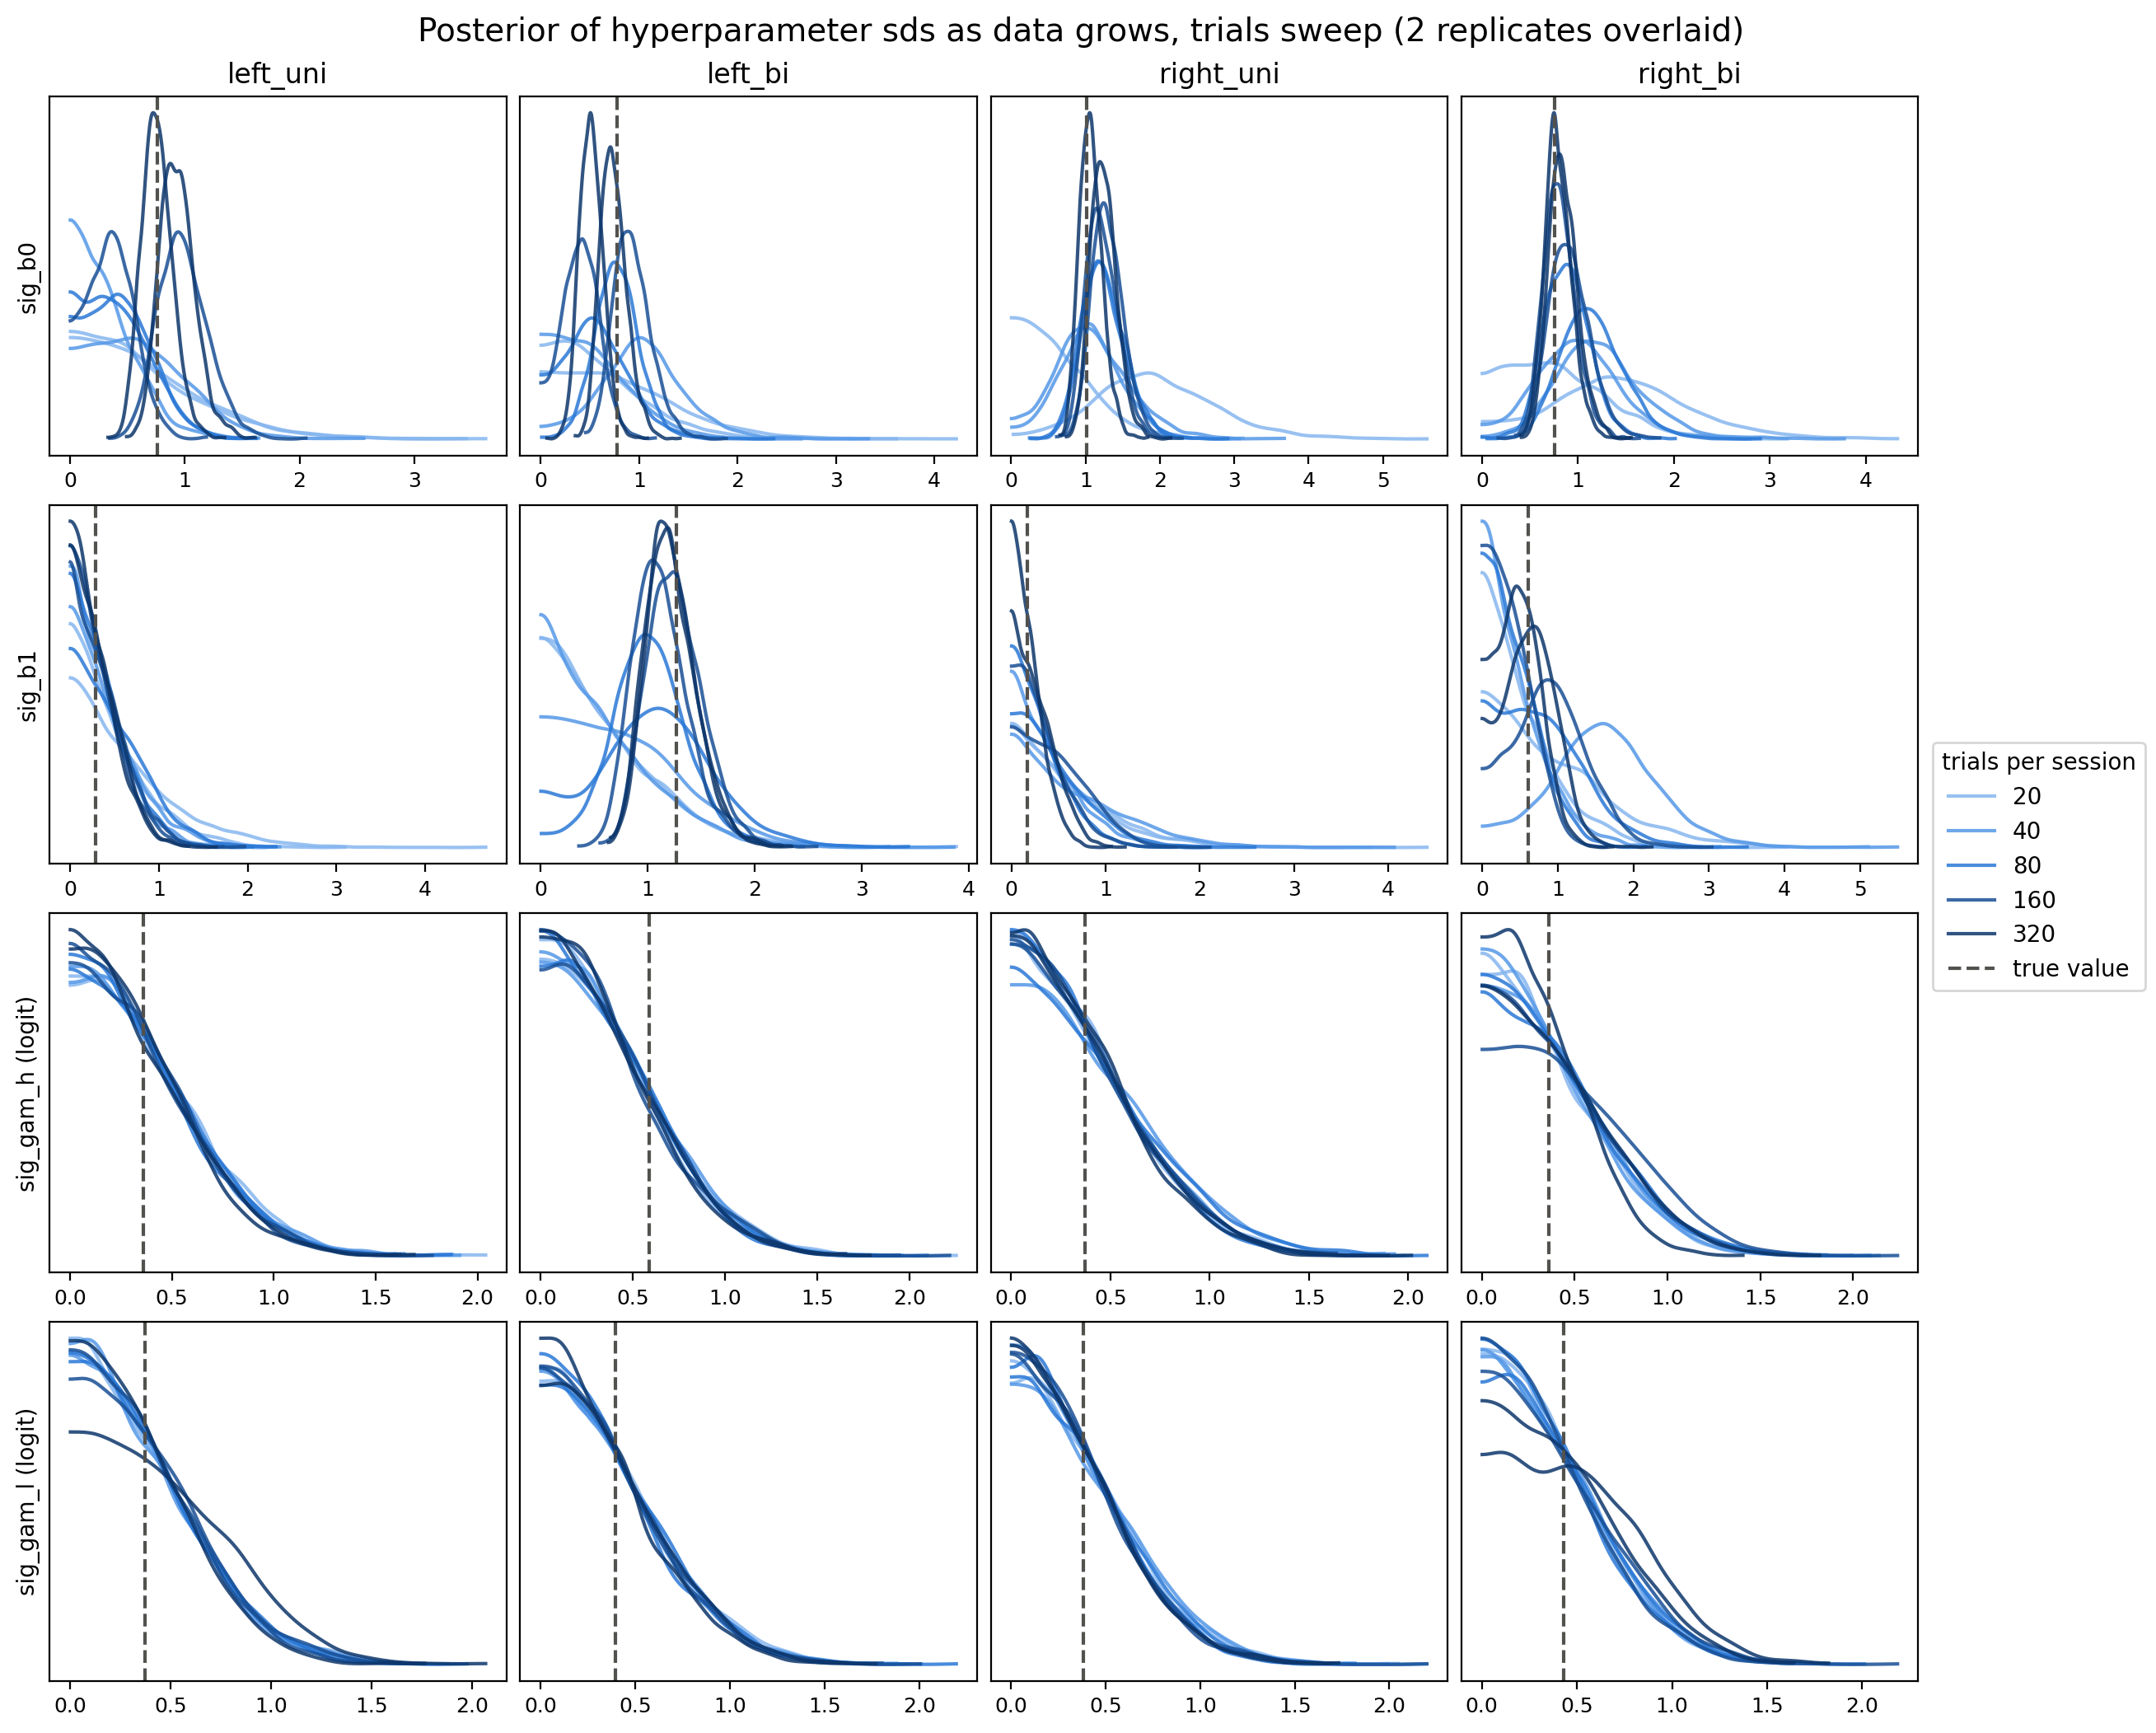
\includegraphics[width=1\linewidth]{hyper_sds_density_vs_trials.png}
    \caption{Posteriors of sd hyperparameters as trials vary}
    \label{fig:sds_density_trials}
\end{figure}

\subsection{Earlier versions of this study}
\label{sec:earlier}

An earlier version of this study used hand-picked true values instead of the real-data
fit: group slopes of 3 (left hand) and 6 (right hand), and between-session sds of the
slope and lapse rates near 0. It was run under both the earlier and the current priors,
on the same synthetic datasets. That comparison motivated the current priors: they
removed the sampling problems of the smallest (5-session) datasets and the truncation
of steep slopes at 8 imposed by the earlier $\mathcal{U}[0, 8]$ prior on
$\mu_{\beta_1}$. Its results are kept in \code{Results\_Convergence\_B\_handpicked.pkl}
(current priors) and \code{Results\_Convergence\_B\_oldpriors.pkl} (earlier priors).
The study reported here replaces it because the hand-picked values did not resemble
the real data, in particular in the slopes and in the between-session sd of the slope.

\subsection{Conclusions for the real data}

At the size of the real dataset (42 sessions of about 308 trials), and at true values
like those estimated from it:

\begin{itemize}
  \item \textbf{Reliable:} per-session PSEs (RMSE about 1.5 $\mu m$, coverage
        0.92--0.98) and JNDs; the group means $\mu_{\beta_0}$ and $\mu_{\beta_1}$; the
        bias spread $\sigma_{\beta_0}$; the slope spread $\sigma_{\beta_1}$ when it is as
        large as that of left\_bi.
  \item \textbf{Weakly determined:} the lapse-rate means, especially $\mu_{\gamma_h}$ of the
        unimanual groups, whose $\gamma_h$ is near 0, and smaller slope spreads
        $\sigma_{\beta_1}$, which cannot be told from 0.
  \item \textbf{Biased in some datasets:} $\mu_{\gamma_l}$ of right\_uni (too high), and the
        lapse rates whose side of the curve does not reach its asymptote: $\gamma_h$ of
        left\_bi (too low) and $\gamma_l$ of left\_uni (too high).
  \item \textbf{Session lapse rates are overconfident:} because $\sigma_{\gamma_h}$ is not
        identified, a miss in a group's $\gamma_h$ carries over to every session, and the
        bimanual session $\gamma_h$ HDIs cover the truth in only 57\% (left) and 86\%
        (right) of sessions. The distractor's effect on $\gamma_h$ in the real data
        should be read at the group level, not session by session.
  \item \textbf{Not identified:} $\sigma_{\gamma_h}$ and $\sigma_{\gamma_l}$. Their posteriors
        largely reflect the priors and should not be interpreted.
  \item The sampler had no difficulties: no divergences in 20 fits.
\end{itemize}

\paragraph{Possible follow-ups.}
\begin{enumerate}
  \item Find out why $\mu_{\gamma_l}$ for right\_uni is overestimated, here and in the
        earlier study.
  \item Consider removing the session-level variation of the lapse rates (one $\gamma_h$
        and $\gamma_l$ per group), since $\sigma_{\gamma_h}$ and $\sigma_{\gamma_l}$ are
        not identified and the session lapse rates are overconfident.
  \item For future experiments: stimulus levels further out would let the curves reach
        their asymptotes and identify the lapse rates.
\end{enumerate}

\end{document}
